\chapter{A Learnable ScatterNet: Locally Invariant Convolutional Layers}

% Specify the path to this folder
\def \path {invariantlayer/}
\def \imgpath {invariantlayer/images}

The drive of this thesis is in exploring if complex wavelets (in
particular the $\DTCWT$) have any place in deep learning and if they do,
quantifying how beneficial they can be. The introduction of more powerful GPUs and
fast and popular deep learning frameworks such as PyTorch, Tensorflow and Caffe
in the past few years has helped the field of deep learning grow very rapidly.
Never before has it been so possible and so accessible to test new designs and
ideas for a machine learning algorithm than today. Despite this rapid growth,
there has been little interest in building wavelet analysis software in modern
frameworks.

This poses a challenge and an opportunity. To pave the way for more detailed
investigation (both in the rest of this thesis and by other researchers
who want to explore wavelets applied to deep learning), we must have the right
foundation and tools to facilitate research.

A good example of this is the current implementation of the ScatterNet. While
ScatterNets have been the most promising start in using wavelets in a deep
learning system, they have tended to be orders of magnitude slower, and significantly more
difficult to run than a standard convolutional network.

Additionally, any researchers wanting to explore the DWT in a deep learning
system have had to rewrite the filter bank implementation themselves, ensuring they
correctly handle boundary conditions and ensure correct filter tap alignment to
achieve perfect reconstruction.

\section{Chapter Layout}
This chapter describes how we have built a fast ScatterNet implementation in
PyTorch with the $\DTCWT$ as its wavelet transform. First, we describe how to do an
efficient DWT in PyTorch in \autoref{sec:ch3:dwt} before showing how to expand this
to an efficient $\DTCWT$ in \autoref{sec:ch3:dtcwt}.
We then use the $\DTCWT$ to define our own ScatterNet in \autoref{sec:ch3:scat} (in
particular, see \autoref{alg:ch3:dtcwt_scat}). 
All of the code is available as an open-source library at \emph{PyTorch Wavelets} \cite{cotter_pytorch_2018}.

In parallel with our efforts, the original authors of the ScatterNet have
improved their implementation, making a new package called KyMatIO\cite{andreux_kymatio:_2018}. 
We compare the speed and classification performance of our package to KyMatIO in \autoref{sec:ch3:comparison}
as this provides some interesting insights into the choice of complex wavelet
for a ScatterNet. This is similar to the work of
\cite{singh_multi-resolution_2016}, where
\citeauthor{singh_multi-resolution_2016} show that a $\DTCWT$-ScatterNet
outperforms a Morlet-ScatterNet when used as a front end to an
SVM for some simpler classification tasks.
We find that our proposed $\DTCWT$-ScatterNet is 7 to 15 times faster 
than KyMatIO (depending on the padding style and wavelet length), as well as
giving a small improvement in performance when used as a front end to a CNN.

\chapter{Introduction}\label{ch:intro}

\def \path {other}
\def \imgpath {\path/images}

It has long been the goal of computer vision researchers to be able to develop
systems that can reliably recognize objects in a scene. Achieving this unlocks a huge
range of applications that can benefit society as a whole: fully
autonomous vehicles, automatic labelling of uploaded videos/images for
searching, interpretation and screening of security video feeds, and many more,
all far-reaching and extremely valuable. Many of these tasks are very tedious for humans
and would be done much better by machines if the missed-detection rate can be
kept low enough. The challenge does not lie in finding the
right application, but in the difficulty of training a computer to see.

Some of the difficulties associated with vision are the presence of nuisance
variables such as changes in lighting condition, changes in viewpoint, and
background clutter. These variables do not affect the scene but can drastically change the pixel
representation of it.
Humans, even at early stages of their lives, have little difficulty filtering
out these nuisance variables and are excellent at extracting the necessary information from a scene.
To design a robust system, it makes sense to take account of how our brains see
and understand scenes.

Unfortunately, biological vision is also a complex system. It has
more to it than simply collecting photons in the eye.
An excerpt from a recent Neurology paper \cite{raichle_two_2010} sums up the problem
well:

\begin{quotation}
It might surprise some to learn that visual information is significantly
degraded as it passes from the eye to the visual cortex. Thus, of the unlimited
information available from the environment, only about $10^{10}$ bits/sec are
deposited in the retina \ldots\ only $\sim 6\times 10^6$
bits/sec leave the retina and only $10^4$ make it to layer IV of V1
\cite{anderson_directed_2005,tor_norretranders_user_1998}. These data
clearly leave the impression that visual cortex receives an impoverished
representation of the world \ldots\ it should be noted that estimates of the
bandwidth of conscious awareness itself (i.e.,\ what we `see') are in the range
of 100 bits/sec or less\cite{anderson_directed_2005,
tor_norretranders_user_1998}.
\end{quotation}

Current video cameras somewhat act as a combination of the first and second
stage of this system, collecting photons in photosensitive sensors and then
converting this to a stream of images. Standard definition digital television
typically has
a bit rate between $3\x 10^6$ and $10^7$ bits/sec (slightly larger but comparable
to the $10^6$ bits/sec travelling through the optic nerve).

If we are to build effective vision systems, it makes sense to emulate this
compression of information between the optic nerve and the later stages of the visual
cortex. 
% The question now stands before us --- what information is kept on entry to the V1 cortex?
Hubel and Wiesel revolutionized our understanding of the V1 cortex in their Nobel prize-winning work
(awarded in 1981 in Physiology/Medicine) by
studying cats \cite{hubel_receptive_1959, hubel_receptive_1962}, macaques and spider
monkeys \cite{hubel_receptive_1968}. They found that neurons in the V1 cortex fired
most strongly when edges of a particular (i.e.,\ neuron-dependent) orientation
were presented to the animal, so long as the edge was inside the receptive field of
this neuron.
Continuing on this work, Blakemore and Cooper \cite{blakemore_development_1970}
analysed the perception of kittens that had restricted visual information
presented to them.
In one of their experiments, the kittens were kept in darkness
and then exposed for a few hours a day to only horizontal or vertical lines.
After five months, they were taken into natural environments and their reactions
were monitored. The two groups of cats would only play with objects when
presented in an orientation that matched the orientation of their original
environment. This suggest that these early layers of perception are
\emph{learned}.
% A figure of the the frequency response of the photoreceptor cells in our eyes
% to different wavelengths of light.
% \begin{figure}
  % \begin{center}
      % 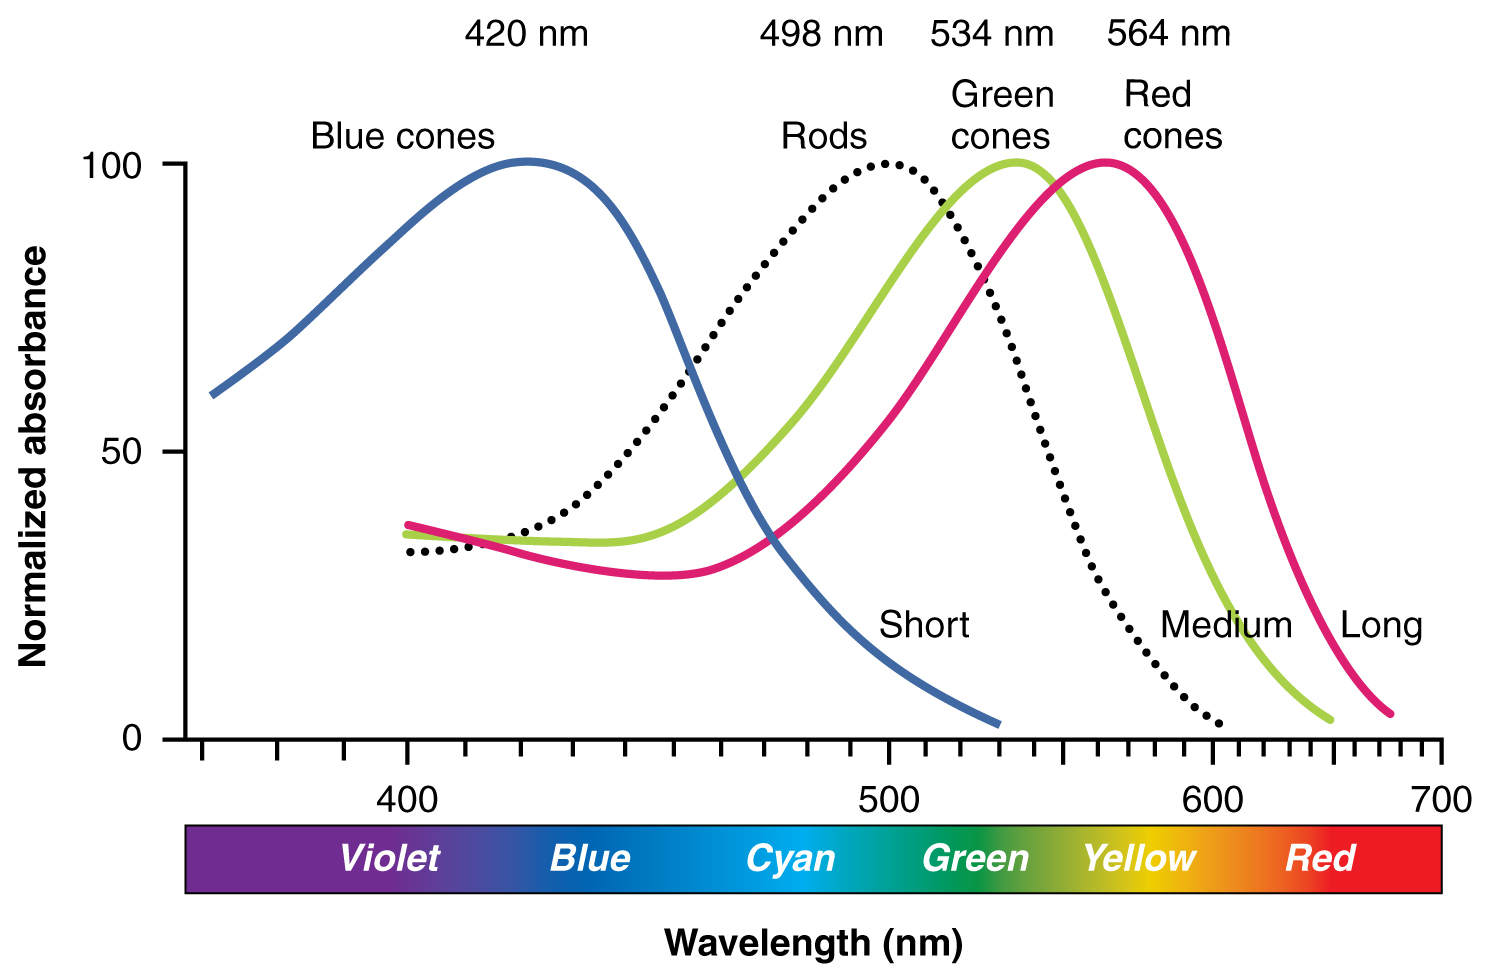
\includegraphics[width=10cm]{\imgpath/colour_sensitivity.jpg}
      % \mycaption{Frequency sensitivity of photoreceptors in they eye}
              % {Wavelength responsiveness of the different photoreceptors in the
               % eye. S, M, and L are short, medium, and long cones, compared to
               % R --- rods. Taken from~\cite{bowmaker_visual_1980}}
  % \end{center}
% \end{figure}

The current state of the art in image understanding systems are
Convolutional Neural Networks (CNNs). These are a learned model that
cascades many convolutional filters serially in layers, separated by
nonlinearities.
They are seemingly inspired by the visual cortex in the way that they are
hierarchically connected, progressively compressing the information into a
richer representation.

\autoref{fig:ch1:cnn_arch} shows an example CNN
architecture, the famous AlexNet \cite{krizhevsky_imagenet_2012}. Inputs are resized to a
manageable size, in this case, $224\x 224$ pixels. Multiple convolutional
filters of size $11\x 11$ are convolved over this input to give $96$ output
\emph{channels} (or \emph{activation maps}). In the figure, these are split onto two
graphics cards or GPUs for memory purposes. These are then passed through a
pointwise nonlinear function, or \emph{nonlinearity}.
The activations are pooled (a form of downsampling) and convolved with more
filters to give $256$ new channels at the second stage. This is repeated 3 more
times until the $13\x 13$ output with $256$ channels is unravelled and passed
through a fully connected neural network to classify the image as one of $1000$
possible classes.

CNNs have garnered lots of attention since 2012 when the previously mentioned AlexNet
nearly halved the top-5 classification error rate (from $26\%$ to $16\%$)
in the ImageNet Large Scale Visual Recognition Competition (ILSVRC)
\cite{russakovsky_imagenet_2014}\footnote{The previous state of
the art classifiers had been built by combining keypoint extractors like
SIFT\cite{lowe_distinctive_2004} and HOG\cite{dalal_histograms_2005} with
classifiers such as Support Vector Machines\cite{cortes_support-vector_1995} and
Fisher Vectors\cite{sanchez_image_2013}, for example \cite{sanchez_high-dimensional_2011}.}.
In the years since, the complexity of CNNs has grown significantly. AlexNet had
only 5 convolutional layers, whereas the 2015 ILSVRC winner ResNet \cite{he_deep_2016}
achieved 3.57\% top-5 error with 151 convolutional layers (and had some
experiments with 1000 layer networks).

\begin{figure}
  \centering
    % \includegraphics[width=\textwidth]{\imgpath/dtcwt_gain}
    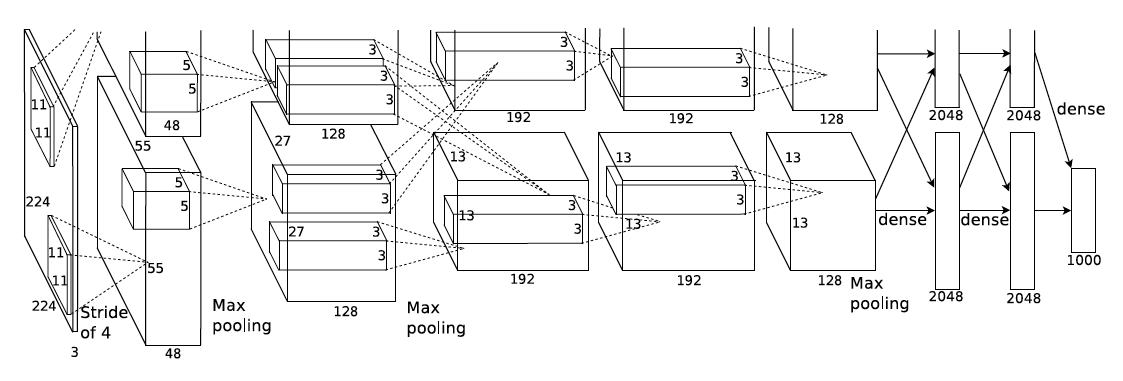
\includegraphics[width=\textwidth]{\imgpath/alexnet.png}
    \mycaption{Convolutional Architecture example}{The previous layer's activations are
    combined with a learned convolutional filter.
    Note that while the activation maps are 3-D arrays, the convolution is only
    a 2-D operation. This means the filters have the same number of channels as
    the input and produce only one output channel. Multiple channels are made by
    convolving with multiple filters. Not shown here are the nonlinearities that
    happen in between convolution operations. Image taken from \cite{krizhevsky_imagenet_2012}.}
    \label{fig:ch1:cnn_arch}
  \end{figure}

\section{Motivation}\label{sec:ch1:motivation}
\begin{figure}
  \centering
  \subfloat[conv1 filters]{
  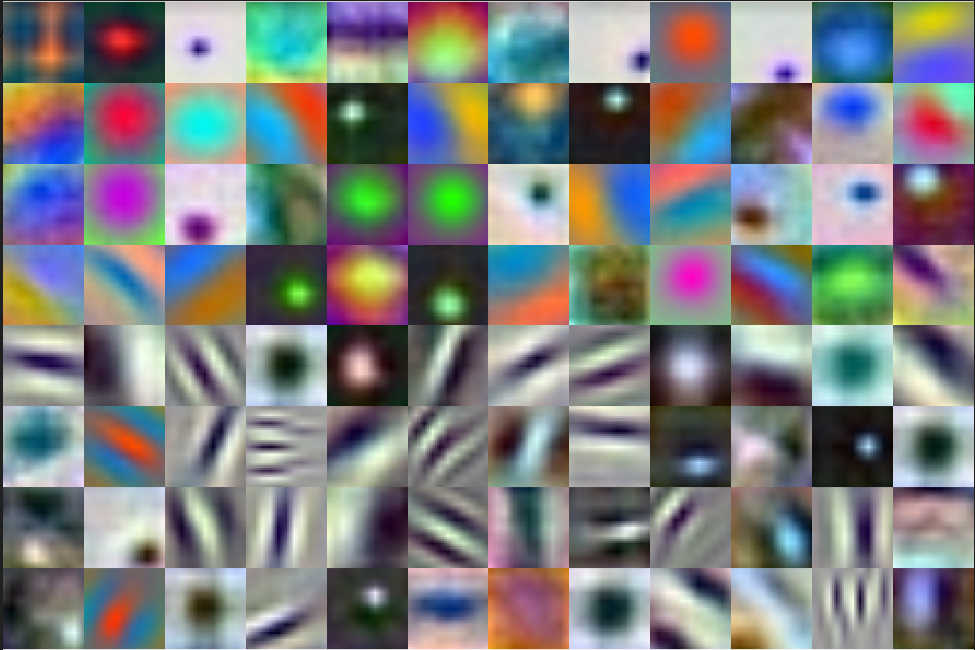
\includegraphics[width=0.6\textwidth]{\imgpath/alexfilters.png}
  \label{fig:ch1:alex_filt}
  }\\
  \subfloat[conv1 activations]{
  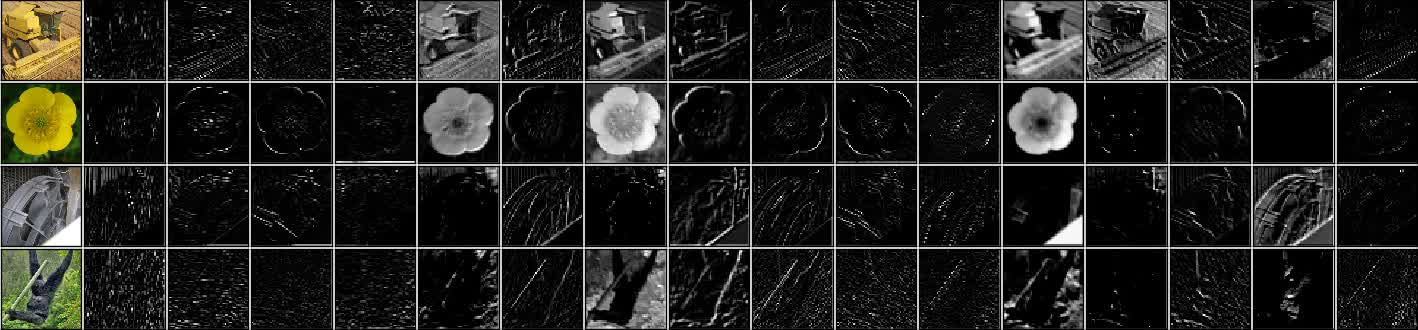
\includegraphics[width=\textwidth]{\imgpath/out1.jpg}
  \label{fig:ch1:alex_conv1}
  }\\
  \subfloat[conv2 activations]{
  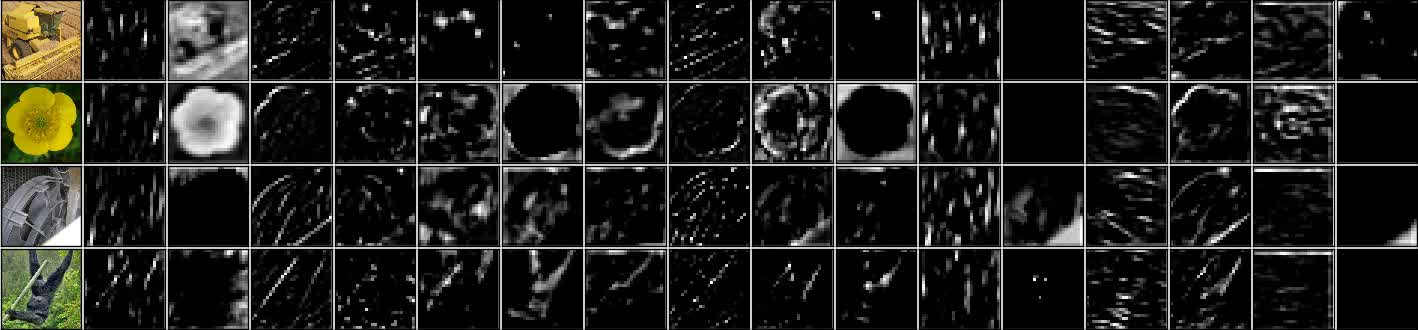
\includegraphics[width=\textwidth]{\imgpath/out2.jpg}
  \label{fig:ch1:alex_conv2}
  }\\
  \subfloat[conv3 activations]{
  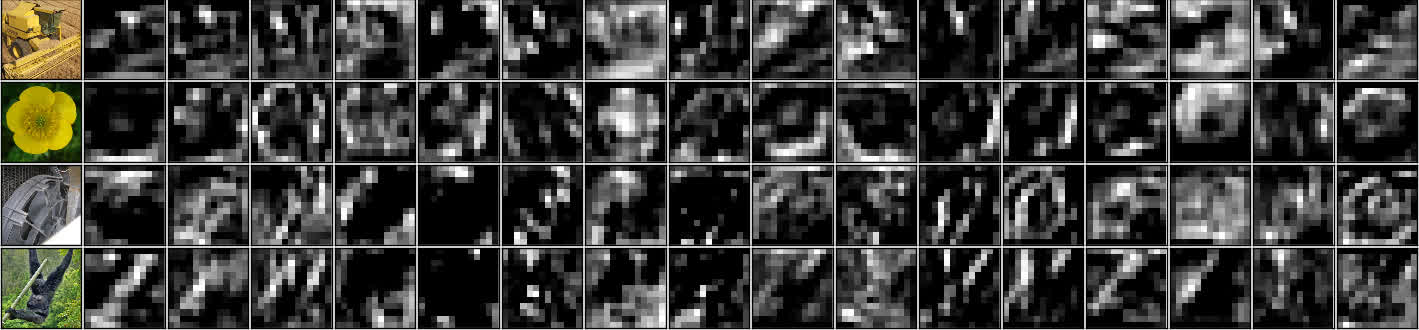
\includegraphics[width=\textwidth]{\imgpath/out3.jpg}
  \label{fig:ch1:alex_conv3}
  }
  \mycaption{Example first layer filters and the first three
  layer's outputs}{\subref{fig:ch1:alex_filt} The $11\x 11$ filters for the
  first stage of AlexNet. Of the 96 filters, 48 were learned on one GPU and
  another 48 on another GPU. Interestingly, one GPU has learned mostly
  lowpass/colour filters and the other has learned oriented bandpass
  filters. \subref{fig:ch1:alex_conv1} - \subref{fig:ch1:alex_conv3} Randomly
  chosen activations from the output of the first, second and third convolutional
  layers of AlexNet (see \autoref{fig:ch1:cnn_arch}) with negative values set to 0.
  Filters and activation images taken from supplementary material of
    \cite{krizhevsky_imagenet_2012}.}
  \label{fig:ch1:alexnet_filters}
\end{figure}

Despite their success, CNNs are often criticized for being \emph{black-box}
methods. You can view the first layer of filters
quite easily (see \autoref{fig:ch1:alex_filt}) as they exist in RGB
space, but beyond that things get trickier as the filters have a third, \emph{channel}
dimension, typically much larger than the two spatial dimensions. Additionally,
it is not clear what the input channels themselves correspond to. For illustration
purposes, we have also shown some example activations from the first three
convolutional layers for AlexNet in
\autoref{fig:ch1:alexnet_filters}\subref{fig:ch1:alex_conv1}-\subref{fig:ch1:alex_conv3}\footnote{These activations are
taken after a specific nonlinearity that sets negative values to 0, hence the
large black regions.}. For the conv1 activations in
\autoref{fig:ch1:alex_conv1}, we can accurately guess that some of the first layer
channels are responding to edges or colour information, but as we go deeper to
conv2 and conv3, it becomes less and less clear what each activation is
responding to.

This has started to become a problem, and while we are happy to trust modern
CNNs for isolated tasks, we are less likely to be comfortable with them driving
cars through crowded cities, or making executive decisions that affect people
directly. In a commonly used contrived example, it is not hard to imagine a deep
network that could be used to assess whether giving a bank loan to an applicant
is a safe investment. Trusting a black box solution is deeply unsatisfactory in
this situation. Not only from the customer's perspective, who, if declined, has
the right to know why \cite{goodman_european_2016}, but
also from the bank's --- before lending large sums of money, most banks
would like to know why the network has given the all clear. `It has worked well
before' is a poor rule to live by.

Aside from their lack of interpretability, it often takes a long time and a lot of
effort to train state-of-the-art CNNs. Typical networks that have won ILSVRC
since 2012 have had roughly 100 million parameters and take up to a week to train. This
is optimistic and assumes that you already know the necessary optimization or
architecture hyperparameters, which you often have to find out by trial and error.
In a conversation the author had with Yann LeCun, the attributed father of
CNNs, at a Computer Vision Summer School (ICVSS 2016), LeCun highlighted this problem
himself:
\begin{quote}
  There are certain recipes (for building CNNs) that work and certain recipes
  that don't, and we don't know why.
\end{quote}

Considering the recent success of CNNs, it is becoming more and more
important to understand \emph{how} and \emph{what} a network learns, so we can
interrogate what in the input has contributed to it making its classification or regression choice.
Without this information, the use of these incredibly powerful tools could be
restricted to research and proprietary applications.

\section{Approach}
The structure of convolutional layers is fairly crude in terms of signal
processing - arbitrary taps of an FIR filter are learned typically via
stochastic gradient descent from random starting states to minimize either a
mean-squared error or cross-entropy loss.

This leads us to ask a motivating question:
%
\begin{quote}
  Is it possible to learn convolutional filters as combinations of basis
  functions rather than individual filter taps?
\end{quote}

In achieving this, it is important to find ways to have an adequate
richness of filtering while reducing the number of parameters needed to specify resulting
filters. We want to contract the space of learning to a subspace or manifold that
is more useful. In much the same way, the convolutional layer in a CNN is a restricted
version of a fully connected layer in a multi-layer perceptron, yet adding this
restriction allowed us to train more powerful networks.

\begin{quote}
The intuition that we explore in this thesis is that \emph{complex wavelets} are
good basis functions for filtering in CNNs.
\end{quote}

\subsection{Why Complex Wavelets?}
Most modern approaches to CNNs are framed entirely in the spatial domain; our
choice of complex wavelets as the basis function to explore comes from the
deeper intuition that it may be helpful to rethink about CNNs in the
\emph{frequency domain}.  Historically, the frequency domain has been an
excellent space for solving many signal processing problems such as noise
removal, filter design, edge detection and data compression. We believe it may prove to
have advantages for CNNs too (beyond just an efficient space to do convolution
in).

The Fourier transform, which uses complex sinusoids as
its basis function, is perhaps the most ubiquitous tool to use for frequency
domain analysis. The problem with these complex sinusoids is that they have
\emph{infinite} support. This means that small changes in one part of an image
affect every Fourier coefficient. Additionally, they are not stable to small
deformations, as small changes can produce unbounded changes in the representation
\cite{mallat_group_2012}.

The common remedy to this problem is to use the localized, and more
stable, short-time Fourier transform (STFT). The STFT (or the Gabor transform)
is a natural extension of the Fourier transform, windowing the complex sinusoids
with a Gaussian (or similar) function. The STFT has the undesirable property that all
frequencies are sampled with the same resolution. A close relative of the STFT is the
continuous wavelet transform (CWT). The shorter duration of the wavelet basis
functions as the frequency increases means that their time resolving power
improves with centre-frequency.
Another commonly used
wavelet transform is the discrete wavelet transform (or the DWT) often favoured over
the CWT because of its speed of computation. It can use many
different finite support basis functions, all with different frequency
localization properties, but it is usually limited to using real filters. As such, it
suffers from many problems such as shift-dependence and lack of directionality in
two dimensions (2-D). These problems can be remedied by using the slower CWT with complex basis
functions, but we choose instead to use the dual-tree complex wavelet transform,
or $\DTCWT$ \cite{selesnick_dual-tree_2005} with q-shift filters \cite{kingsbury_complex_2001}.

The $\DTCWT$ allows for complex basis functions that have shift-invariance and
directionality, while being fast to implement like the DWT (in 2-D it can be thought of as the
application of 4 DWTs in parallel). It is also more easily invertible than the
CWT, forming a tight frame \cite{kovacevic_introduction_2008}, which we believe
may prove to be a very important property for visualizing what a
CNN is responding to.

We revisit the properties of the Fourier transform, STFT, CWT, DWT and $\DTCWT$
and expand on the properties behind our choice of basis functions
in the literature review \autoref{sec:ch2:fourier}.

On top of the intuition that the wavelet domain is a good space in which to frame CNNs,
there are some experimental motivating factors too. Firstly, the wavelet
transform has had much success in image and video compression, particularly for
JPEG2000 \cite{taubman_jpeg2000_2013}. Good compression performance implies an ability of
the basis functions to represent the input data sparsely (as seems to happen in
the brain). Secondly, the filters from the first layer of AlexNet
(\autoref{fig:ch1:alexnet_filters}) look like oriented wavelets. Given that
there was no prior placed on the filters to make them have this similarity to
wavelets, this result is noteworthy. And finally, the aforementioned work of
Hubel and Wiesel suggests that the early layers of the visual system act like a
Gabor transform.

These experimental observations imply that complex wavelets would do well in
replacing the first layer of a CNN, but we would aslo like to find out if they can be used
at deeper layers. Their well-understood and well-defined behaviour would help us
to answer the above \emph{how} and \emph{why} questions. Additionally, they
allow us to enforce a certain amount of smoothness and near orthogonality;
smoothness seems to be important to avoid sensitivity to adversarial or spoofing
attacks \cite{szegedy_intriguing_2014} and near orthogonality allows you to
cover a large space with fewer coefficients.

But first, we must find out \emph{if} it is possible to get the same or nearly the same
performance by using wavelets as the building blocks for CNNs, and this is the
core goal of this thesis.

\section{Method}
\subsection{ScatterNets}
To explore the uses of complex wavelets in CNNs, we begin by looking at one of the most
popular current uses of wavelets in image recognition tasks, the
Scattering Transform.

The Scattering Transform, or the \emph{ScatterNet}, was introduced in \cite{mallat_group_2012,
bruna_invariant_2013} at the same time as AlexNet. It is a non-black-box
network that can be thought of as a restricted complex-valued CNN
\cite{bruna_mathematical_2015}. Unlike a CNN, it has predefined
convolutional kernels, set to complex wavelet (and scaling) functions and uses
the complex magnitude as its nonlinearity. Due to
its well-defined structure, it can be analyzed and bounds on its stability to
shifts, noise and deformations are found in \cite{mallat_group_2012}.
%
% This is a promising start to addressing the problems of CNNs as using
% predefined, general filters helps us answer \emph{how} a CNN is
% learning, although the \emph{what} is still somewhat unclear.

For a simple task like identifying small handwritten digits,
the variabilities in the data are simple and small and the ScatterNet can easily
reduce the problem into a space which a Gaussian Support Vector Machine (or SVM
\cite{cortes_support-vector_1995}) can easily solve
\cite{bruna_invariant_2013}. For a more complex task like identifying real-world
objects, the ScatterNet can somewhat reduce the variabilities and get good
results with an SVM, but there is a significant performance gap between this and
what a CNN can achieve. For example, in \cite{oyallon_deep_2015} a second-order
ScatterNet can achieve $82.3\%$ top-1 classification accuracy on CIFAR-10, a
commonly used dataset, whereas modern CNNs such as \cite{he_deep_2016} can
achieve $93.4\%$.

\subsection{Learnable ScatterNets}
To start to address the performance gap between ScatterNet front ends and CNNs
we first investigate the properties of current ScatterNets. Inspired by the
visualization work of \citeauthor{zeiler_visualizing_2014}
\cite{zeiler_visualizing_2014} we build a DeScatterNet. The DeScatterNet
leverages the perfect reconstruction properties of the $\DTCWT$ and allows us to
investigate what in the input image the ScatterNet is responding to.

The DeScatterNet shows that the ScatterNet may be limiting itself by not
combining the filtering of different wavelet orientations (it does not mix the
channels as a CNN does). Inspired by the work of \cite{qiu_dcfnet:_2018}, we
propose the learnable ScatterNet, which includes this mixing while keeping the
desirable properties of the ScatterNet.

The learnable ScatterNet can be thought of as using the scattering outputs as
the \emph{basis functions}\footnote{Although they are not true basis functions
as they are the combination of a complex wavelet with a modulus nonlinearity,
and are thus data-dependent.} for our convolutional layers. We show that this
improves greatly on the ScatterNet design, and under certain constraints can
improve on the performance of CNNs too.

\subsection{Wavelet Domain Filtering}
We find that the complex modulus of the ScatterNet design to be useful for some
operations in a CNN, but it has a demodulating effect on the frequency energy
(all the outputs have significantly more energy in lower frequencies). This
limits repeated application of it as the demodulating effect compounds.

We develop a system that does not use the complex modulus; instead, it
learns \emph{complex} gains in the wavelet domain.
Rather than mixing subbands together, we keep them independent and only learn to
mix across the channel dimension. This is important, as it allows us to then use the inverse
$\DTCWT$ to return to the pixel domain. The shift-invariant properties of the $\DTCWT$ mean the
reconstructed outputs are (mostly) free from aliasing effects, despite much of
the processing being carried out at significantly reduced sample rates in the
wavelet domain.

We show that our layer can be used alongside regular convolutional
layers. I.e., it becomes possible to `step' into the wavelet domain to do
wavelet filtering for one layer, before `stepping' back into the pixel domain to
do pixel filtering for the next layer.

\section{Thesis Layout and Contributions to Knowledge}
This thesis has one literature review chapter and four novel-work chapters:
\begin{itemize}
\item
  \hyperref[ch:litreview]{Chapter~\ref*{ch:litreview}}
  explores some of the background necessary for starting
  to develop image understanding models. In particular, it covers the
  inspiration for CNNs and the workings of CNNs themselves, as well as covering
  the basics of wavelets and ScatterNets.
\item
  \Autoref{Chapter}{ch:dtcwt_scat} proposes a change to the core of the ScatterNet. In
  addition to performance issues with ScatterNets, they are slow and both
  memory-intensive and compute-intensive to calculate. This in itself is enough of an
  issue to make it unlikely that they would be used as part of deep networks. To
  overcome this, we change the computation to use the $\DTCWT$
  \cite{selesnick_dual-tree_2005} instead of Morlet wavelets, achieving a 20 to
  30 times speed-up while achieving a small improvement in classification performance.
\item
  \Autoref{Chapter}{ch:visualizing} describes our \emph{DeScatterNet}, a tool used to
  interrogate the structure of ScatterNets. We also perform tests to determine
  the usefulness of the different scattered outputs finding that many of them
  are not useful for image classification.
\item
  \Autoref{Chapter}{ch:invariant} describes the \emph{Learnable ScatterNet} we have developed to
  address some of the issues found from the interrogation in
  \autoref{ch:visualizing}. We find that a learnable ScatterNet layer performs
  better than a regular ScatterNet, and can improve on the performance of a CNN
  if used instead of pooling layers. We also find that scattering works well not
  just on RGB images, but can also be useful when used after one layer of
  learning.
\item
  In \autoref{ch:freqlearn}, we step away from ScatterNets and present the
  \emph{Wavelet Gain Layer}. The gain layer uses
  the wavelet space as a latent space to learn representations. We find possible
  nonlinearities and describe how to learn in both the pixel and wavelet domain.
  This work showed that there may well be benefits to learning in the wavelet
  domain for earlier layers of CNNs, but we have not yet found advantages to
  using the wavelet gain layer for deeper layers.
\end{itemize}

\subsection{Contributions and Publications}
The key contributions of this thesis are:

\begin{itemize}
  \item Software for wavelets and $\DTCWT$ based ScatterNet (described in \autoref{ch:dtcwt_scat})
    and publicly available at \cite{cotter_pytorch_2018}.
  \item ScatterNet analysis and visualizations (described in
    \autoref{ch:visualizing}). This chapter expands on the paper we presented at MLSP2017
    \cite{cotter_visualizing_2017}.
  \item Invariant Layer/Learnable ScatterNet (described in \autoref{ch:invariant})). This chapter expands
    on the paper accepted at ICIP2019 \cite{cotter_learnable_2019}. Software
    available at \cite{cotter_learnable_2019-1}.
  \item Learning convolutions in the wavelet domain (described in
    \autoref{ch:freqlearn}). We have published preliminary results on this work
    to arXiv \cite{cotter_deep_2018} but have expanded on this paper in the
    chapter. Software available at \cite{cotter_dtcwt_2018}.
\end{itemize}

\subsection{Related Research}
Readers may also be interested in the theses \cite{singh_scatternet_2018} and
\cite{oyallon_analyzing_2017}.

In \cite{singh_scatternet_2018}
\citeauthor{singh_scatternet_2018} looks at using the ScatterNet as a fixed
front end and combining it with well-known machine learning methods such as
SVMs, Autoencoders and Restricted Boltzmann Machines. By combining frameworks in
a defined way he creates unsupervised feature extractors which can then be used
with simple classifiers. Some relevant papers that makeup this thesis are \cite{singh_multi-resolution_2016,
singh_scatternet_2017, singh_generative_2018}. In
\cite{singh_multi-resolution_2016} Singh shows
that the $\DTCWT$-ScatterNet outperforms a Morlet-ScatterNet when used as a front end for
an SVM, which is similar to the work we do in \autoref{ch:dtcwt_scat} where we
show the $\DTCWT$-ScatterNet outperforms a Morlet-ScatterNet when used as a
front end for CNNs. He then expands on this work by testing other backends in
\cite{singh_scatternet_2017, singh_generative_2018}.

In \cite{oyallon_analyzing_2017}
\citeauthor{oyallon_analyzing_2017} looks at ScatterNets as front ends to
deeper learning systems, such as CNNs. Some relevant papers that makeup Oyallon's thesis are
\cite{oyallon_deep_2015, oyallon_scaling_2017, oyallon_hybrid_2017}. \cite{oyallon_scaling_2017, oyallon_hybrid_2017}
are particularly relevant as he uses a ScatterNet as a feature extractor for a
CNN. We do similar research in \autoref{ch:invariant}, but allow for
learned weights in the ScatterNet in our design.

\section{Related Work}\label{sec:ch5:related}

There have been several similar works that look into designing new convolutional
layers by separating them into two stages --- a first stage that performs a
non-standard filtering process, and a second stage that combines the first stage
into single activations. The inception layer 
\cite{szegedy_rethinking_2015} by \citeauthor*{szegedy_rethinking_2015} does this by filtering with different
kernel sizes in the first stage, and then combining with a $1\x 1$ convolution
in the second stage. \citeauthor*{ioannou_training_2015} also do something similar by making
a first stage with horizontal and vertical filters, and then combining in the
second stage again with a $1\x 1$ convolution\cite{ioannou_training_2015}. But perhaps the most similar
works are those that use a first stage with fixed filters, combining them in a
learned way in the second stage. Of particular note are:
\begin{itemize}
\item 
\citetitle{juefei-xu_local_2016} \cite{juefei-xu_local_2016}. This paper builds a
first stage with a small $3\x 3$ kernel filled with zeros, and randomly insert
$\pm 1$ in several locations, keeping a set sparsity level. This builds a very
crude spatial differentiator in random directions. The output of the first stage
is then passed through a sigmoid nonlinearity before being mixed with a $1\x 1$
convolution. The imposed structure on the first stage was found to be a good
regularizer and prevented overfitting, and the combination of the mixing in the
second layer allowed for a powerful and expressive layer, with performance near
that of a regular CNN layer.

\item
``DCFNet: Deep Neural Network with Decomposed Convolutional Filters"
\cite{qiu_dcfnet:_2018}. This paper decomposes convolutional filters as linear
combinations of Fourier Bessel and random bases.  The first stage projects the
inputs onto the chosen basis, and the second stage learns how to mix these
projections with a $1\x 1$ convolution. Unlike \cite{juefei-xu_local_2016} this
layer is purely linear. The supposed advantage being that the
basis can be truncated to save parameters and make the input less susceptible to
high frequency variations. The work found that this layer had marginal benefits
over regular CNN layers in classification, but had improved stability to noisy
inputs. 

\end{itemize}

\section{Recap of Useful Terms}\label{sec:ch5:background}

\subsection{Convolutional Layers}\label{sec:ch5:conv}

Let the output of a CNN at layer $l$ be 
$ \cnnlact{x}{l}{c}{\xy}, \quad c\in \{0, \ldots C_l-1\}, \xy \in \reals[2]$
where $c$ indexes the channel dimension, and $\xy$ is a vector of coordinates
for the spatial position. Of course, $\xy$ is typically sampled on a grid, but
we keep it continuous to more easily differentiate between the spatial and
channel dimensions. Recall from \eqref{eq:ch2:conv4} and \eqref{eq:ch2:conv4a} that
a convolutional layer in a standard CNN is defined by the two operations:
%
\begin{eqnarray} 
  \cnnlact{y}{l+1}{f}{\xy} &=& \sum_{c=0}^{C_l - 1}  x^{(l)}(c,\xy) \conv h^{(l)}_{f}(c, \xy)
    \label{eq:ch5:conv}\\
    \cnnlact{x}{l+1}{f}{\xy} & = & \sigma \left( \cnnlact{y}{l+1}{f}{\xy} \right) \label{eq:ch5:nonlin}
\end{eqnarray}

where $\cnnfilt{l}{f}{c}{\xy}$ is the $f$th filter of the $l$th layer with $C_l$
different point spread functions, and $f \in \{0, \ldots, C_{l+1}-1 \}$. $\sigma$ is a nonlinearity 
such as the ReLU, possibly combined with scaling such as batch normalization. The convolution
is done independently for each $c$ in the $C_l$ channels and the resulting outputs are
summed together to give one activation map. 

\subsection{Wavelet Transforms}\label{sec:ch5:wavelets}
Recall from \eqref{eq:ch2:wave2} that:
\begin{equation}
  \mathcal{W}x(c, \xy) = \left\{x(c, \xy) \ast \phitd_J(\xy),\ x(c, \xy) \ast \psitd_{\lambda}(\xy) \right\}_{\lambda} \label{eq:ch5:wave2}
\end{equation}
Where $\psitd_\lambda$ is a mother wavelet dilated by $2^j,\ 1 \leq j \leq J$ and rotated by
$\theta = \frac{\pi + 2k\pi}{12},\ 0\leq k < 6$:
%
\begin{equation}
  \psi_{j, \theta}(\xy) = 2^{-j}\psi \left(2^{-j} r_{-\theta} \xy\right)
\end{equation}
Define the set of all possible $\lambda$s as $\Lambda$ whose size is $|\Lambda | = JK$.
%
\subsection{Scattering Transforms}\label{sec:ch5:scatter}
As the real and imaginary parts of complex wavelets are in quadrature with
each other, taking the modulus of the resulting transformed coefficients removes
the high frequency oscillations of the output signal while preserving the energy
of the coefficients over the frequency band covered by $\psi_\lambda$. This is
crucial to ensure that the scattering energy is concentrated towards
zero-frequency as the scattering order increases, allowing sub-sampling.
% We experimentally show in \autoref{sec:??} that it plays a vital role in the
%classification process. 
We define the wavelet modulus propagator to be:
%
\begin{equation}
  \label{eq:ch5:wave_mod}
\widetilde{\mathcal{W}}x(c, \xy) = \left\{ x(c, \xy) \conv \phi_{J}(\xy),\ |x(c, \xy) \conv \psi_\lambda (\xy) | \right\}_{\lambda \in \Lambda} 
\end{equation}
The modulus terms are called $U[\lambda] x = \lvert x \conv \psi_\lambda \rvert$, and the scattering terms
are $S[\lambda] x = U[\lambda]x \conv \phi_J (\xy)$.

\section{The Scattering Transform} \label{sec:ch4:scatternet}
While we have introduced the scattering transform before, we clarify the format
we use for this chapter's analysis.

We use the $\DTCWT$ based ScatterNet introduced in the previous chapter --
\autoref{alg:ch3:dtcwt_scat} as a front end, with $K=6$ orientations, $J=2$
scales and $M=2$ orders.

Consider a single-channel input signal $x(\xy)$, $\xy \in \reals[2]$.
The zeroth-order scatter coefficient is the lowpass output of a $J$
level filter bank:
%
\begin{equation}
  S_0x(\xy) \definedas x(\xy) \conv \phi_J(\xy)
\end{equation}
%
This is approximately invariant to translations of up to $2^J$ pixels\footnote{From here on,
we drop the $\xy$ notation when indexing $x$, for clarity.}. In exchange for
gaining invariance, the $S_0$ coefficients have lost information
(contained in the rest of the frequency space). The remaining energy of $x$ is
contained within the first-order \emph{wavelet} coefficients:
\begin{equation}
  W_1x(\lambda_1, \xy) \definedas x \conv \psi_{\lambda_1}
\end{equation}
for $\lambda_1 = (j_1, \theta_1)$, $j_1\in\{1, 2\}, \theta_1 = \frac{\pi +
2k\pi}{12}$ with $k \in \{0, 1, \ldots 5\}$.

Taking the magnitude of $W_1$ gives us the first-order \emph{propagated}
signals:
\begin{equation}
  U_1x(\lambda_1, \xy) \definedas |x \conv \psi_{\lambda_1}|
    = \sqrt{(x \conv \psi^r_{\lambda_1})^2 + (x \conv \psi^i_{\lambda_1})^2}
\end{equation}
The first-order scattering coefficient make $U_1$ invariant up to
the coarsest scale $J$ by averaging it:
\begin{equation}
  S_1x(\lambda_1, \xy) \definedas |x \conv \psi_{\lambda_1}| \conv \phi_J
\end{equation}
This has $KJ = 6\x 2 = 12$ output channels for each input channel. Later in this
chapter we will want to distinguish between the first and second scale
coefficients of the $S_1$ terms, which we will do by moving the $j$ index
to a superscript. I.e., $S_1^1$ and $S_1^2$ refer to the set of 6 $S_1$ terms
at the first and second scales.

The second-order scattering coefficients are defined only on paths of
decreasing frequency (i.e. $J_2 < J_{1}$) \cite{bruna_invariant_2013}
\begin{equation}
  S_2x(\lambda_1, \lambda_2, \xy) \definedas |U_1x \conv \psi_{\lambda_2}| \conv \phi_J \label{eq:ch4:s2}
\end{equation}
Previous work shows that for natural images we get diminishing returns after
$m=2$. Our output is then a stack of these 3 outputs:
\begin{equation}
  Sx = \{S_0x, S_1x, S_2x\}
\end{equation}
with $1+12+36=49$ channels per input channel.

\subsection{Scattering Colour Images}\label{sec:ch4:colour}
A wavelet transform like the $\DTCWT$ accepts single-channel input yet we
often work on RGB images. This leaves us with a choice. We can either:
\begin{enumerate}
  \item Apply the wavelet transform (and the subsequent scattering operations)
    on each channel independently. This would triple the output size to $3C$.
  \item Define a frequency threshold below which we keep colour information, and
    above which, we combine the three channels.
\end{enumerate}
The second option uses the well known fact that the human eye is far less sensitive
to higher spatial frequencies in colour channels than in luminance channels.
This also fits in with the first layer filters seen in the well known
Convolutional Neural Network, AlexNet. Roughly one half of the filters were low
frequency colour `blobs', while the other half were higher frequency, greyscale,
oriented wavelets.

For this reason, we choose the second option for the
architecture described in this chapter. We keep the 3 colour
channels in our $S_0$ coefficients but work only on greyscale for high orders
(the $S_0$ coefficients are the lowpass bands of a J-scale wavelet transform, so
we have effectively chosen a colour cut-off frequency of $2^{-J} \frac{f_s}{2}$).

We combine the three channels by modifying our magnitude operation from \eqref{eq:ch3:magbias}
to now be:
\begin{equation}\label{eq:ch4:colour_mag}
 r_s = \sqrt{x_r^2 + y_r^2 + x_g^2 + y_g^2 + x_b^2 + y_b^2 + b^2} - b
\end{equation}
Where $x_r, x_g, x_b$ are the real parts of the wavelet response for the red,
green and blue channels, and $y$ is the corresponding imaginary part. This only
affects the $S_1$ coefficients and the $S_2$ coefficients then are calculated
as per \eqref{eq:ch4:s2}.

An alternative to \eqref{eq:ch4:colour_mag} is to combine the colours
\emph{before} scattering into a luminance channel. However, we choose to use \eqref{eq:ch4:colour_mag}
instead as this has the ability to detect colour edges with constant luminance.

With $J=2$ the resulting scattering output now has $3 + 12 + 36 = 51$ channels at $1/16$ the
spatial input size.

\section{The Inverse Scatter Network}\label{sec:ch4:descatternet}
\begin{figure}[t]
  \centering
  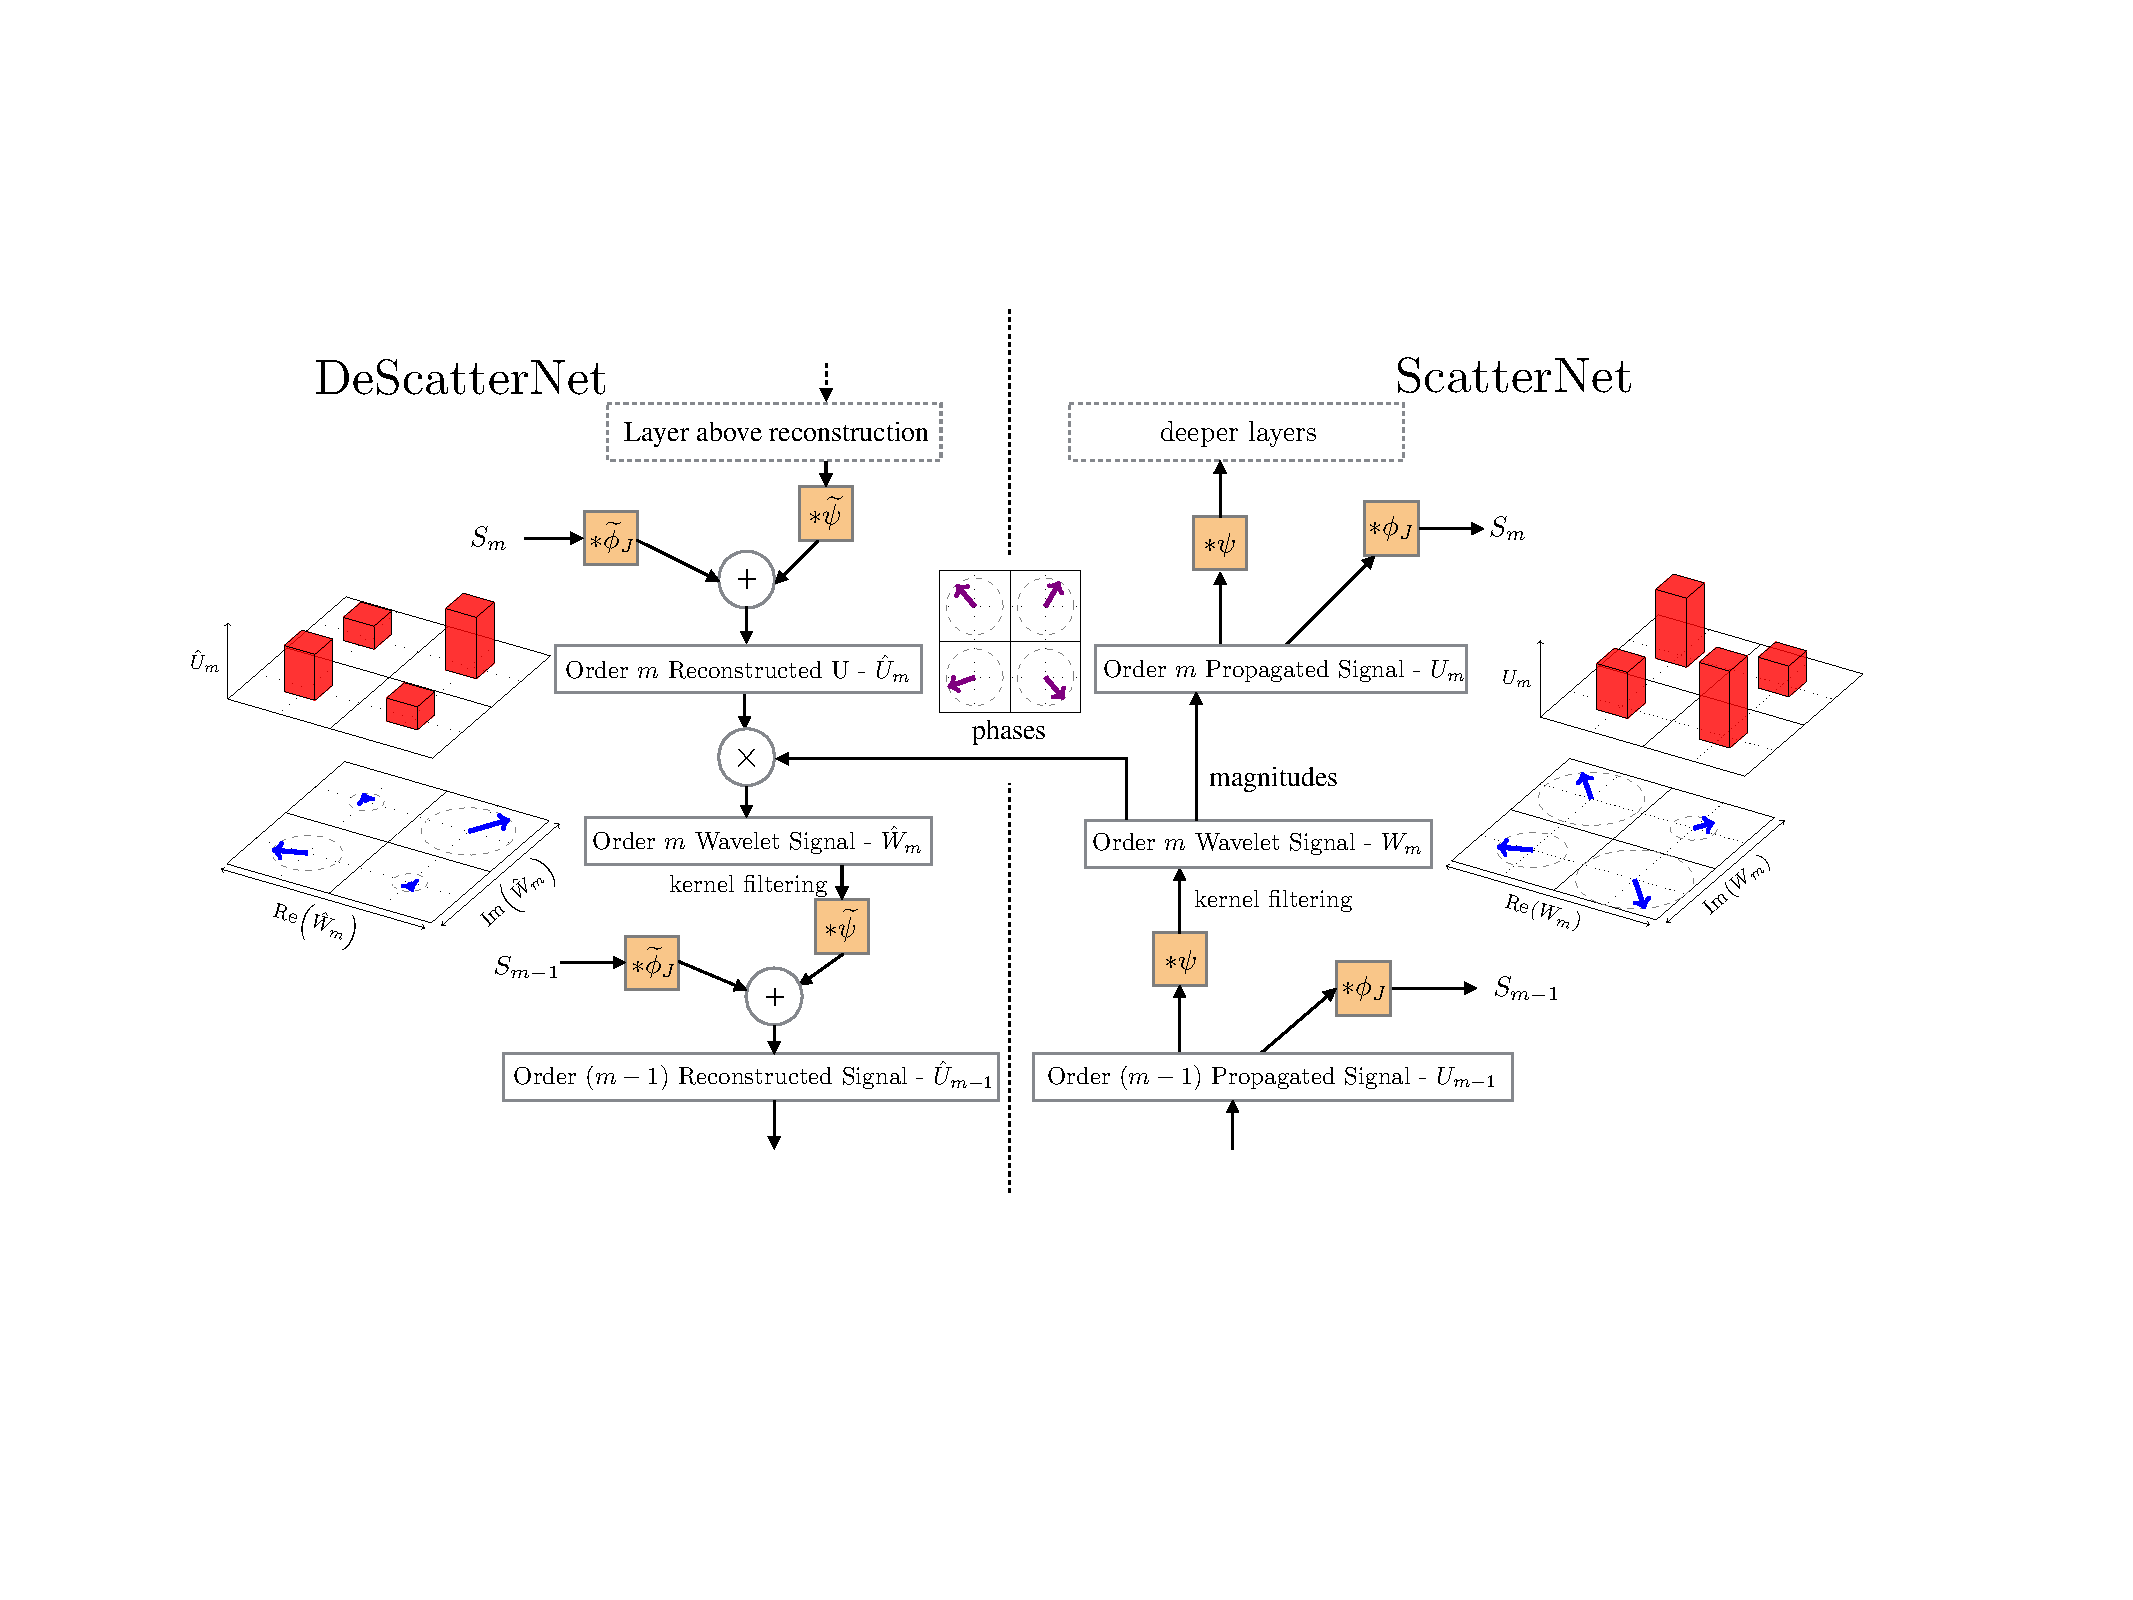
\includegraphics[width=\textwidth, trim={3cm 7cm 4cm 6cm},clip]{\imgpath/descat.pdf}
  \mycaption{The inverse scattering network}{Comprises a DeScattering layer (left)
  attached to a Scattering layer (right). We are using the same convention as
  \cite{zeiler_visualizing_2014} Figure 1 - i.e., the input signal starts in the
  bottom right-hand corner, passes forwards through the ScatterNet (up the right
  half), and then is reconstructed in the DeScatterNet (downwards on the left
  half). The DeScattering layer will reconstruct an approximate version of the
  previous order's propagated signal. The $2\x 2$ grids shown around the image
  are either Argand diagrams representing the magnitude and phase of small
  regions of \emph{complex} (De)ScatterNet coefficients or bar charts showing
  the magnitude of the \emph{real} (De)ScatterNet coefficients (after applying
  the modulus nonlinearity). For reconstruction, we need to save the discarded
  phase information and reintroduce it by multiplying it with the reconstructed
  magnitudes.}
  \label{fig:ch4:descat}
\end{figure}

We now introduce our inverse scattering network. This allows us to back-project
scattering coefficients to the image space; it is inspired by the
DeconvNet used by Zeiler and Fergus in
\cite{zeiler_visualizing_2014} to look into the deeper layers of CNNs. Like
the DeConvNet, the inverse scattering network is similar to backpropagating a
single strong activation (rather than the usual gradient terms).

We emphasize that instead of thinking about perfectly reconstructing $x$ from
$S\in \reals[C\x H'\x W']$, we want to see what signal/pattern in the input image caused
a large activation in each channel. This can then give us a good idea of what each
output channel is sensitive to, or what the ScatterNet is `extracting' from the input.
Note that we do not use any of the log normalization layers described in
\cite{oyallon_deep_2015, singh_dual-tree_2017}.

\subsection{Inverting the Low-Pass Filtering}
Going from the $U$ coefficients to the $S$ coefficients in the forward pass involves convolving by
a low pass filter $\phi_J$, possibly followed by decimation to make the output $(H\x
2^{-J})\x (W\x2^{-J})$.  $\phi_J$ is a purely real filter, and we can `invert'
this operation by interpolating $S$ to the same spatial size as $U$ and convolving with
the mirror image of $\phi_J$, $\widetilde{\phi}_J$ (this is equivalent to the
transpose convolution described in \cite{zeiler_visualizing_2014}).
\begin{equation}
  \label{eq:ch4:s_hat}
  \hat{S}_{m}x = (S_{m}x) \conv \widetilde{\phi}_J
\end{equation}
% This will not recover $U$ as it was on the forward pass, but will recover all
% the information in $U$ that caused a strong response in $S$.
We note that
interpolation usually involves lowpass smoothing of the signal, so this can all
be one operation.
% However this has
% the undesirable effect of creating multiple impulses in the next layer down's
% activations. When the next layer down is the image space this is not a problem,
% but when it is

\subsection{Inverting the Magnitude Operation}
In the same vein as \cite{zeiler_visualizing_2014}, we face a difficult
task in inverting the nonlinearity in our system.
% It has been proven that for
% particular wavelets, we can recover the phase from their modulus
% \cite{waldspurger_phase_2012}, but this is not a trivial operation. Instead, we
We lend inspiration from the switches introduced in the DeconvNet; the
switches in a DeconvNet save the location of maximal activations so that
on the backwards pass activation layers could be unpooled trivially. We do an
equivalent operation by saving the \emph{phase} of the complex activations.
On the backwards pass we reinsert the phase\footnote{We note that this is equivalent 
to finding the gradient through the magnitude operation, just as the `switches' 
from \cite{zeiler_visualizing_2014} are equivalent to taking the gradient of 
the max pooling layer.} to give our recovered $W$:
\begin{equation}
  \label{eq:ch4:w_hat}
  \hat{W}_{m}x = \left(\hat{U}_{m} x\right) e^{j\theta_{m}}
\end{equation}

\subsection{Inverting the Wavelet Decomposition}
Using the $\DTCWT$ makes inverting the wavelet transform simple, as we
can simply feed the coefficients through the synthesis filter banks to regenerate
the signal. For complex $\psi$, this is convolving with the conjugate transpose
$\widetilde{\psi}$:
\begin{eqnarray}
  \label{eq:ch4:x_hat}
  \hat{U}_{m-1}x &=& \hat{S}_{m-1}x + \hat{W}_{m}x \\
                 &=& (S_{m-1}x) \conv \widetilde{\phi}_J + \sum_{\lambda_m} \left(\hat{U}_m x\right) e^{j\theta_m}
  \conv \widetilde{\psi}_{\lambda_m}
\end{eqnarray}

\subsection{The $\DTCWT$ ScatterNet}
The combination of the above three stages can be repeated for higher orders. The
resulting DeScatterNet is shown in \autoref{fig:ch4:descat}.

For the $\DTCWT$ ScatterNet (from \autoref{alg:ch3:dtcwt_scat}), this is the same
as finding the \emph{gradient} from the corresponding channels in $Z$.

\section{Visualization with Inverse Scattering}
{
\renewcommand{\_}{\textscale{.6}{\textunderscore}}
\label{sec:ch4:visualization}

We scatter all of the images from ImageNet's validation set and record the top 9
images which most highly activate each of the $C$ channels in the ScatterNet.
This is the \emph{identification} phase (in which no inverse scattering is
performed).

Then, in the \emph{reconstruction} phase, we load in the $9\x C$ images and
scatter them one by one. We take the resulting 52 channel output vector and mask
all but the largest value in the channel we are currently
examining and mask all values in the other channels.
This 1-sparse tensor is then presented to the inverse scattering network from
\autoref{fig:ch4:descat} and projected back to the image space.

Some results of this are shown in \autoref{fig:ch4:reconstructions} for the
first and second-order coefficients. For a given output channel, we show the top
9 activations projected independently to pixel space. We also show the patch
of pixels in the input image which cause this large output. As there are 12
$S_1$ coefficients, we randomly choose 3 orientations from $S_1^1$ and 3 from $S_1^2$.
Similarly, there are 36 $S_2$ coefficients, so we randomly choose 16 of these.

The order 0 and order 1 scattering (labelled with `Order 1' in
\autoref{fig:ch4:reconstructions}) coefficients look quite similar to the first
layer filters from the well-known AlexNet CNN \cite{krizhevsky_imagenet_2012}.
This is not too surprising, as the first-order scattering coefficients are
simply a wavelet transform followed by average pooling. They are responding to
images with strong edges aligned with the wavelet orientation.

The second-order coefficients (labelled with `Order
2' in \autoref{fig:ch4:reconstructions}) appear very similar to the order
1 coefficients at first glance.
They too are sensitive to edge-like features, and some of them (e.g.\ third row,
third column and fourth row, second column) are mostly just that. These are
features that have the same oriented wavelet applied at both the first and
second-order ($\theta_1 = \theta_2$). Others, such as the nine in the top left
square (first row, first column), and top right square (first row, fourth
column) are more sensitive to checker-board like patterns. These are
activations where the orientation of the wavelet for the first and second-order
scattering were far from each other ($15\degs$ and $105\degs$ for the first row,
first column and $105\degs$ and $45\degs$ for the first row, fourth column).

For comparison, we include reconstructions from the second layer of the
well-known VGG CNN\@ (labelled with `VGG conv2\_2', in
\autoref{fig:ch4:reconstructions}). These were made with a DeconvNet, following the
same method as \cite{zeiler_visualizing_2014}. Note that while some of
the features are edge-like, we also see higher-order shapes like corners,
crosses and curves.

These reconstructions show that higher-order features from ScatterNets vary
significantly from those learned in CNNs. In many
respects, the features extracted from a CNN like VGGNet look preferable for use
as part of a classification system.
\begin{figure}[tp]
  \centering
  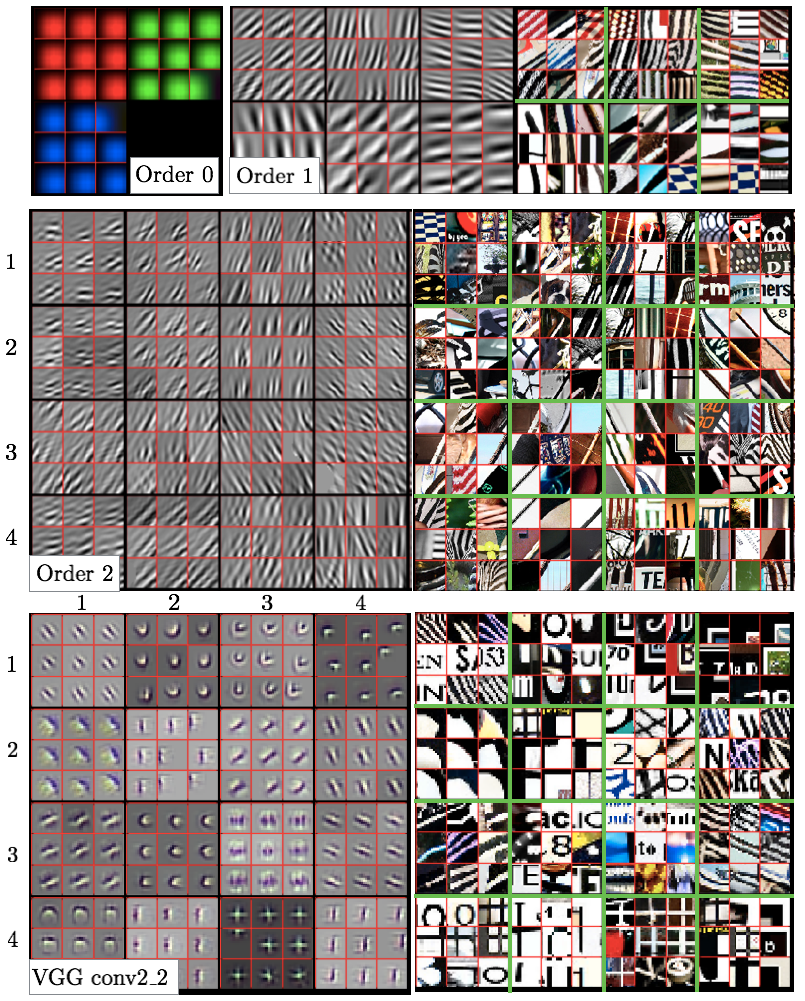
\includegraphics[width=0.9\textwidth]{\imgpath/deconv_images.png}
  \mycaption{Comparison of scattering to convolutional features}{Visualization
  of a random subset of features from $S_0$ (all 3), $S_1$ (6 from the 12) and
  $S_2$ (16 from the 36) scattering outputs. We record the top 9 activations for
  the chosen features and project them back to the pixel space. We show them
  alongside the input image patches which caused the large activations. We also
  include reconstructions from layer conv2\_2 of VGG Net
  \cite{simonyan_very_2014}(a popular CNN, often used for feature extraction)
  for reference --- here we display 16 of the 128 channels. The VGG
  reconstructions were made with a CNN DeconvNet based on
  \cite{zeiler_visualizing_2014}. Image best viewed digitally.}
  \label{fig:ch4:reconstructions}
\end{figure}

}

\section{Implementation Details}\label{sec:implementation}
Again, we use the $\DTCWT$ \cite{selesnick_dual-tree_2005} for our wavelet filters
$\psi_{j, \theta}$ due to their fast implementation with separable convolutions
which we will discuss more in \autoref{sec:computation}.  There are two side
effects of this choice. The first is that the number of orientations of wavelets
is restricted to $K=6$. The second is that we naturally downsample the output
activations by a factor of $2$ for each direction for each scale $j$, giving a 
$4^j$ downsampling factor overall. This represents the
source of the invariance in our layer. If we do not wish to downsample the
output (say to make the layer fit in a larger network), we can bilinearly
interpolate the output of our layer. This is computationally cheap to do on its
own, but causes the next layer's computation to be higher than necessary (there
will be almost no energy for frequencies higher than $f_s/4$).

In all our experiments we set $J=1$ for each invariant layer,
meaning we can mix the lowpass and bandpass coefficients at the same resolution.
\autoref{fig:block_diagram} shows how this is done. Note that setting $J=1$ for
a single layer does not restrict us from having $J>1$ for the entire system, as
if we have a second layer with $J=1$ after the first, including downsampling
($\downarrow$), we would have:
%
\begin{equation}
  \left(\left(\left(x \conv \phi_1\right) \downarrow 2\right) \conv \psi_{1, \theta}\right) 
    \downarrow 2 = \left(x \conv \psi_{2, \theta}\right) \downarrow 4
\end{equation}

\subsection{Parameter Memory Cost}\label{sec:memory}
A standard convolutional layer with $C_l$ input channels, $C_{l+1}$ output channels
and kernel size $L\x L$ has $L^2C_{l}C_{l+1}$ parameters. 

The number of learnable parameters in each of our proposed invariant layers with
$J=1$ and $K=6$ orientations is:
%
\begin{equation}
  \text{\#params} = (JK+1)C_{l}C_{l+1} = 7C_{l}C_{l+1}
\end{equation} 
%
The spatial support of the wavelet filters is typically $5\x 5$ pixels or more,
and we have reduced $\text{\#params}$ to less than $3\x3$ per filter, while
producing filters that are significantly larger than this.

\subsection{Activation Memory Cost}
A standard convolutional layer needs to save the activation $x^{(l)}$ to
convolve with the backpropagated gradient $\dydx{L}{y^{(l+1)}}$ on the backwards
pass (to give $\dydx{L}{w^{(l)}}$). For an input with $C_l$ channels of spatial size $H\x W$, this means
$HWC_l$ floats must be saved. 

Our layer requires us to save the activation
$z^{(l+1)}$ for updating the $\tilde{a}$ terms. This has $7C_l$ channels of
spatial size $\frac{HW}{4}$. This means that our proposed layer needs to save
$\frac{7}{4}HWC_l$ floats, a $\frac{7}{4}$ times memory increase on the standard
layer.

\begin{algorithm}[tb]
\caption{Locally Invariant Convolutional Layer forward and backward
passes}\label{alg:ch6:inv}
\begin{algorithmic}[1]
\Procedure{GAINLAYERFWD}{$x,\ g_{lp},\ g_1$}
\State $u_{lp},\ u_{1} \gets \DTCWT(x^l, \mbox{nlevels}=1) $ \Comment{$u_{1}$ has 6 orientations and is complex}
  \State \textbf{save} $u_{lp},\ u_{1}$ \Comment{For the backwards pass}
  \State $v_{lp} \gets u_{lp} \conv g_{lp}$ 
  \For{$1\leq k \leq 6$}
  \State \begin{varwidth}[t]{\linewidth}  $v_{1,k} \gets 
      \left( \real{u_{1,k}} \conv \real{g_{1,k}} - \imag{u_{1,k}} \conv \imag{g_{1,k}} \right)\ +$ \par
      \hskip\algorithmicindent \hphantom{abc}$ j\left(\real{u_{1,k}} \conv \imag{g_{1,k}} + \imag{u_{1,k}} \conv \real{g_{1,k}}\right)$;
  \end{varwidth}
  \EndFor
  \State $y \gets \DTCWT^{-1}(v_{lp}, v_{1})$
  \State \textbf{return} $y$
\EndProcedure
\end{algorithmic}\vspace{10pt}
\begin{algorithmic}[1]
  \Procedure{GAINLAYERBWD}{$\dydx{L}{Y},\ g_{lp},\ g_1$}
  \State \textbf{load} $u_{lp},\ u_1$
  \State \textbf{return} $\dydx{L}{x},\ \dydx{L}{A}$
\EndProcedure
\end{algorithmic}
\end{algorithm}



\subsection{Computational Cost}\label{sec:computation}
A standard convolutional layer with kernel size $L\x L$ needs $L^2C_{l+1}$
multiplies per input pixel (of which there are $C_{l}\x H\x W$).

As mentioned in \autoref{sec:memory}, we use the $\DTCWT$ for our complex, shift
invariant wavelet decomposition. We use the open source Pytorch implementation
of the $\DTCWT$ \cite{cotter_pytorch_2018} as it can run on GPUs and
has support for backpropagating gradients.

There is an overhead in doing the wavelet decomposition for each input channel.
A separable 2-D discrete wavelet transform (DWT) with 1-D filters of length $L$
will have $2L\left(1-2^{-2J}\right)$ multiplies per input pixel for a $J$ scale
decomposition. A $\DTCWT$ has 4 DWTs for a 2-D input, so its cost is
$8L\left(1-2^{-2J}\right)$, with $L=6$ a common size for the filters. It is
important to note that unlike the filtering operation, this does not scale with
$C_{l+1}$, the end result being that as $C_{l+1}$ grows, the cost of $C_l$
forward transforms is outweighed by that of the mixing process whose cost is
proportional to $C_l C_{l+1}$.

Because we are using a decimated wavelet decomposition, the sample rate
decreases after each wavelet layer. The benefit of this is that the mixing
process then only works on one quarter the spatial size after the first scale
and one sixteenth the spatial after the second scale. Restricting ourselves to
$J=1$ as we mentioned in \autoref{sec:implementation}, the computational cost is
then:

\begin{equation}
  % \frac{7}{4}C_{l+1} + 48 \label{eq:comp}
  \underbrace{ \frac{7}{4}C_{l+1} }_{\textrm{mixing}} +
  \underbrace{\vphantom{\frac{7}{4}} 36}_{\DTCWT} \quad
  \textrm{multiplies per input pixel}\label{eq:ch5:comp}
\end{equation}
In most CNNs, $C_{l+1}$ is several dozen if not several
hundred, which makes \eqref{eq:ch5:comp} significantly smaller than
$L^2C_{l+1}=9C_{l+1}$ multiplies for $3\x 3$ convolutions.

\subsection{Forward and Backward Algorithm}
There are two layer hyperparameters to choose in our layer:
\begin{itemize}
  \item The number of output channels $C_{l+1}$. This may be restricted by the
    architecture.
  \item The variance of the weight initialization for the mixing matrix $A$.
\end{itemize}

Assuming we have already chosen these values, 
then the forward and backward algorithms can be computed with
Algorithm~\autoref{alg:ch5:inv}.


\section{Experiments}\label{sec:experiments}
In this section we examine the effectiveness of our invariant layer by testing
its performance on the well known datasets (listed in the order of increasing
difficulty):
\begin{itemize}
  \item MNIST: 10 classes, 6000 images per class, $28\x 28$ pixels per image.
  \item CIFAR-10: 10 classes, 5000 images per class, $32\x 32$ pixels per image.
  \item CIFAR-100: 100 classes, 500 images per class, $32\x 32$ pixels per image. 
  \item Tiny ImageNet\cite{li_tiny_nodate}: 200 classes, 500 images per class, 
    $64 \x 64$ pixels per image. 
\end{itemize}
Our experiment code is available at
\url{https://github.com/fbcotter/invariant_convolution}.

\subsection{Layer Introduction with MNIST}\label{sec:ch5:mnist}
To begin experiments on the proposed locally invariant layer, we look at how
well a simple system works on MNIST, and compare it to an equivalent system with
convolutions. To minimize the effects of learning from other layers, we build a
custom small network, as described in \autoref{tab:ch5:mnist_arch}.

The first two layers are learned convolutional/invariant layers, followed by
a fully connected layer with fixed weights that we can use to project down to
the number of output classes. Finally, we add a small learned layer that
linearly combines the 10 outputs from the random projection, to give 10 new
outputs. This is to facilitate reordering of the outputs to the correct class.
This simple network is meant to test the limits of our layer, rather than
achieve state of the art performance on MNIST.

Given that our layer is quite different to a standard convolutional layer, we
must do a full hyperparameter search over optimizer parameters such as the
learning rate, momentum, and weight decay, as well layer hyperparameters 
such as the variance of the random initialization for the mixing matrix $A$.

To simplify the weight variance search, we use Glorot Uniform Initialization
\cite{glorot_understanding_2010} and only vary the gain value $a$:
%
\begin{equation}
  A_{ij} \drawnfrom U\left[ -a\sqrt{\frac{6}{(C_l + C_{l+1})HW}},\ a\sqrt{\frac{6}{(C_l + C_{l+1})HW}}\
  \right] \label{eq:ch5:glorot}
\end{equation}
%
where $C_l,\ C_{l+1}$ are the number of input and output channels as before, and
the kernel size is $H = W = 1$ for an invariant layer and $H = W= 3$ for a
convolutional layer.

We do a grid search over these hyperparameters and use Hyperband
\cite{li_hyperband:_2016} to schedule early stopping of poorly performing runs.
Each run has a grace period of 5 epochs and can train for a maximum of 20
epochs. We do not do any learning rate decay.  We found the package Tune
\cite{liaw2018tune} was very helpful in organising parallel distributed training
runs.  
% Finally, we use fANOVA \cite{hutter_efficient_2014} analysis
% to find the importance of these hyperparameters to our layer, comparing to a
% standard layer. 
The hyperparameter options are described in
\autoref{tab:ch5:hyper_options}, note that we test $4^4=256$ different options.

Once we find the optimal hyperparameters for each network, we then run the two
architectures 10 times with different random seeds and report the mean and variance of
the accuracy. The results of these runs are listed in
\autoref{tab:ch5:mnist_initial_results}.

\begin{table}[t]
  \renewcommand{\arraystretch}{1.4}
  \centering
  \mycaption{Architectures for MNIST hyperparameter experiments}{The activation
  size rows are offset from the layer description rows to convey the input and
  output shapes. The `project' layers in both architectures are unlearned, so all
  of the learning has to be done by the first two layers and the reshuffle
  layer.}
  \label{tab:ch5:mnist_arch}
  \subfloat[Reference Arch with $3\x 3$ convolutions]{%
    \label{tab:ch5:mnist_arch_conv}
    \begin{tabular}{c c}
      \toprule
      Activation Size & Layer Name + Info \\
      \midrule
      \begin{tabular}{@{}c@{}} % This supresses the space on the left and right
        $1\x 28 \x 28$ \\ $7\x 28\x 28$ \\ $7\x 14\x 14$ \\ $49\x 14\x 14$ \\ $49\x 7\x 7$ 
        \\ $2401\x 1$ \\ $10\x 1$ \\ $10\x 1$ 
      \end{tabular} &
      \begin{tabular}{@{}c@{}}
        conv1, $w \in \reals[7\x 1\x 3 \x 3]$ \\ maxpool1, $2\x 2$ \\ 
        conv2 $w \in \reals[49\x 7 \x 3\x 3]$ \\ maxpool2, $2\x 2$ \\ unravel \\
        project, $w \in \reals[2401\x 10]$ \\ reshuffle, $w\in \reals[10\x 10]$
      \end{tabular} \\
      \bottomrule
    \end{tabular}
  }\quad
  \subfloat[Invariant Architecture]{%
    \label{tab:ch5:mnist_arch_inv}
    \begin{tabular}{c c}
      \toprule
      Activation Size & Layer Name + Info \\
      \midrule
      \begin{tabular}{@{}c@{}} % This supresses the space on the left and right
        $1\x 28 \x 28$ \\ $7\x 14\x 14$ \\ $49\x 7\x 7$ \\ $2401\x 1$ \\ $10\x 1$
        \\ $10\x 1$ 
      \end{tabular} &
      \begin{tabular}{@{}c@{}}
        inv1, $A \in \reals[7\x 7]$ \\ inv2, $A \in \reals[49\x 49]$ \\ unravel \\
        project, $w \in \reals[2401\x 10]$ \\ reshuffle, $w\in \reals[10\x 10]$
      \end{tabular}\\
      \bottomrule
    \end{tabular}
  }
\end{table}




\begin{table}[hbt]
  \centering
  \mycaption{Hyperparameter settings for the MNIST experiments}{The weight gain is
  the term $a$ from \autoref{eq:ch5:glorot}. Note that $\log_{10} 3.16 = 0.5$.}
  \label{tab:ch5:hyper_options}
  \begin{tabular}{c c}
    \toprule
    Hyperparameter & Values \\
    \midrule
    Learning Rate (lr) & $\left\{ 0.0316,\ 0.1,\ 0.316,\ 1 \right\}$ \\
    Momentum (mom) & $\left\{ 0,\ 0.25,\ 0.5,\ 0.9 \right\}$ \\
    Weight Decay (wd) & $\left\{ 10^{-5},\ 3.16\x 10^{-5},\ 10^{-4},\ 3.16\x 10^{-4} \right\} $\\
    Weight Gain (a) & $\left\{0.5,\ 1.0,\ 1.5,\ 2.0 \right\}$
    \\\bottomrule
  \end{tabular}
\end{table}

\begin{table}[hbt]
  \centering
  \mycaption{Architecture performance comparison}{Numbers reported are the mean
  and standard deviation of accuracy over 10 runs with the optimal
  hyperparameters, $\theta$. Note that for
  both architectures we found that $\F{lr}$ was the most important
  hyperparameter to choose correctly, and had the largest impact on the
  performance.
  % We also use
  % fANOVA\cite{hutter_efficient_2014} analysis to weight the importance of these 
  % hyperparameters. High values imply the accuracy is more sensitive to this
  % hyperparameter. 
  }
  \label{tab:ch5:mnist_initial_results}
  \begin{tabular}{@{}l c c c@{}}
    \toprule
     & &\multicolumn{2}{c}{accuracy} \\\cline{3-4}
    Architecture & $\theta = \{\F{lr}, \F{mom}, \F{wd}, \F{a}\}$ & mean & std  \\\midrule
    Convolutional & $\{0.1,\ 0.5,\ 10^{-5},\ 1.5 \}$ & 97.3 & 0.29 \\
    Invariant & $\{0.032,\ 0.9,\ 3.2\x 10^{-5},\ 1.0 \}$ & 96.6 & 0.26 \\
    \bottomrule
  \end{tabular}
\end{table}


\subsubsection{Proposed Expansions}\label{sec:ch5:mnist_initial}
The results from the previous section seem to indicate that our proposed
invariant layer is a slightly worse substitute for a convolutional layer.
However we believe that this is due to the centred nature of the wavelet bases
that were used to generate the $z$ and later the $y$ coefficients. A similar
effect was seen in the previous chapter in \autoref{fig:ch4:shapes} where the
space of shapes attainable by mixing wavelet coefficients in a $3\x 3$ area was
much richer than those attainable by only mixing in a $1\x 1$ area. 

To test this hypothesis, we change \autoref{eq:ch5:mixing} to be:
\begin{equation}
  y^{(l+1)}(f, \xy)  =  \sum_{q \in Q} z^{(l+1)}(q, \xy) \conv \left(\tilde{a}_f(q) \alpha_f(q, \xy) \right)
\end{equation}

Where $\alpha_f(q, \xy)$ is an introduced kernel designed to allow mixing of
wavelets from neighbouring spatial locations. We test a range of possible
$\alpha$'s each with varying complexity/overhead:

\begin{enumerate}[(a)]
  \item We randomly shift each of the $7C$ subbands horizontally
    by $\{-1, 0, 1\}$ pixels, and vertically by $\{-1, 0, 1\}$ pixels. This is
    determined at the beginning of a training session and is consistent between
    batches. This theoretically is free to do, but practically it involves
    convolving with a $3 \x 3$ kernel with a single $1$ and eight $0$'s.
  \item Instead of shifting impulses as in the previous option, we can shift a
    gaussian kernel by one pixel left/right and up/down, making a smoother filter. 
  \item Instead of imposing a lowpass/impulse structure, we can set $\alpha$ to
    be a random $3\x 3$ kernel. This is chosen once at the beginning of training and then
    is kept fixed between batches.
  \item We can set the $3\x 3$ kernel to be fully learned. This
    still makes for a novel layer, but now the parameter cost is 9 times higher
    than the $1\x 1$ conv layer, and 7 times higher than a vanilla $3\x 3$
    convolution.
  \item We can take the top three $3\x 3$ DCT coefficients of the $7C$
    subbands, allowing us to do something like the previous option 
    but with only a threefold parameter increase. The top three coefficients are
    the constant, the horizontal and the vertical filters.
\end{enumerate}

Again, we search over the hyperparameter space to find the optimal
hyperparameters and then run 10 runs at the best set of hyperparameters, and
report the results in \autoref{tab:ch5:mnist_new_results}. As we expected,
adding in random shifts significantly helps the invariant layer. Two systems of
note are the shifted impulse (a) system and the learned $3\x 3$ kernel (d)
system. The first improves the mean accuracy by $1.3\%$ without any extra
learning. The second improves the performance by $2.4\%$ but with a large
parameter cost. To explore an equivalent system, we also list in
\autoref{tab:ch5:mnist_new_results} a modification to the convolutional
architecture that uses $5\x 5$ convolutions and $C_1 = 10,\ C_2 = 100$ channels,
resulting in a system with comparable parameter cost to (d).

\begin{table}[hbt]
  \renewcommand{\arraystretch}{1.4}
  \centering
  \mycaption{Modified architecture performance comparison}{Numbers reported are the mean
  and standard deviation of accuracy over 10 runs with the optimal
  hyperparameters, $\theta$. We also list parameter cost and number
  of multiplies for each layer option, relative to the standard $3\x 3$
  convolutional layer to highlight the benefits/drawbacks of each option.}
  \label{tab:ch5:mnist_new_results}
  \begin{tabular}{@{}l c c c c c@{}}
    \toprule
    & & \multicolumn{2}{c}{cost} & \multicolumn{2}{c}{accuracy} \\\cline{3-4}\cline{5-6}
    Architecture & $\theta = \{\F{lr}, \F{mom}, \F{wd}, \F{a}\}$ & param & mults & mean & std  \\\midrule
    Convolutional & $\{0.1,\ 0.5,\ 10^{-5},\ 1.5 \}$ & 1 & 1 & 97.3 & 0.29 \\
    Invariant & $\{0.032,\ 0.9,\ 3.2\x 10^{-5},\ 1.0 \}$ & $\frac{7}{9}$ & $\frac{7}{36}$ & 96.6 & 0.26 \\\midrule
    Shifted impulses (a) & $\{0.32,\ 0.5,\ 10^{-4},\ 1.0 \}$ & $\frac{7}{9}$ & $\frac{7}{36}$ & 97.9 & 0.25 \\
    Shifted gaussians (b) & $\{1.0,\ 0.0,\ 10^{-5},\ 1.0 \}$ & $\frac{7}{9}$ & $\frac{7}{4}$ & 97.7 & 0.56\\
    Random $3\x3$ kernel (c) & $\{1.0,\ 0.9,\  10^{-5},\ 1.0 \}$ & $\frac{7}{9}$ & $\frac{7}{4}$ & 95.8 & 1.01\\
    Learned 3 DCT coeffs (d) & $\{1.0,\ 0.0,\ 10^{-5},\ 1.0 \}$ & $\frac{7}{3}$ & $\frac{7}{4}$ & 98.1 & 0.37\\\midrule
    Learned $3\x3$ kernel & $\{0.1,\ 0.5,\  10^{-4},\ 1.0 \}$ & \textbf{7} & $\frac{7}{4}$ & \textbf{99.0} & 0.12 \\\midrule
    Wide Convolutional & $\{0.32,\ 0.5,\ 10^{-5},\ 1.5 \}$ & 7 & 7 & 98.7 & 0.25  \\
    \bottomrule
  \end{tabular}
\end{table}


\subsection{Layer Comparison with CIFAR and Tiny ImageNet}\label{sec:conv_exp}
Now we look at expanding our layer to harder datasets, focusing more on the
final classification accuracy. We do this again by comparing to a reference
architecture. For this task, we choose a VGG-like network as our reference.
It has six convolutional layers for CIFAR and eight layers for Tiny ImageNet as shown in
\autoref{tab:arch}. The initial number of channels $C$ we use is 64. Despite
this simple design, this reference architecture achieves competitive performance
for the three datasets.

We perform an ablation study where we progressively swap out convolutional
layers for invariant layers keeping the input and output activation sizes the
same. As there are 6 layers (or 8 for Tiny ImageNet), there are too many
permutations to list the results for swapping out all layers for our locally
invariant layer, so we restrict our results to swapping 1 or 2 layers. 
\autoref{tab:conv_results} reports the top-1 classification accuracies for
CIFAR-10, CIFAR-100 and Tiny ImageNet. In addition to testing on the full
datasets we report results for a reduced training set size. In the table, `invX'
means that the `convX' layer from \autoref{tab:arch} is replaced with an 
invariant layer.

This network is optimized with stochastic gradient descent with momentum. The
initial learning rate is $0.5$, momentum is $0.85$, batch size $N=128$ and
weight decay is $10^{-4}$. For CIFAR-10/CIFAR-100 we scale the learning rate by
a factor of 0.2 after 60, 80 and 100 epochs, training for 120 epochs in total.
For Tiny ImageNet, the rate change is at 18, 30 and 40 epochs (training for 45 in total).

\begin{table}[t]
  \renewcommand{\arraystretch}{1.4}
  \centering
  \mycaption{CIFAR and Tiny ImageNet Base Architecture}{Reference architecture
  used for experiments on CIFAR-10, CIFAR-100 and Tiny ImageNet. This
  architecture is based off the VGG\cite{simonyan_very_2014} architecture. $C$ is a
  hyperparameter that controls the network width, we use $C=64$ for our initial
  tests. The activation size rows are offset from the layer description rows to
  convey the input and output shapes.}
  \label{tab:ch5:cifar_tiny_arch}
  \subfloat[CIFAR Architecture]{%
    \label{tab:ch5:cifar_arch}
    \begin{tabular}{l l}
      \toprule
      Activation Size & Layer Name + Info \\
      \midrule
      \begin{tabular}{@{}l@{}} % This supresses the space on the left and right
        $3\x 32\x 32$ \\ $C\x 32\x 32$ \\ $C \x 32\x 32$ \\ $C\x 16\x 16$ \\
        $2C\x 16 \x 16$ \\ $2C\x 16\x 16$ \\ $2C\x 8\x 8$ \\
        $4C\x 8\x 8$ \\ $4C\x 8\x 8$\\ $4C\x 1\x 1$ \\
        $10\x1$, $100\x1$ 
      \end{tabular} &
      \begin{tabular}{@{}l@{}}
        convA, $w \in \reals[C\x 3\x 3\x 3]$ \\       
        convB, $w \in \reals[C\x C\x 3\x 3]$ \\       
        pool1, max pooling $2\x 2$ \\
        convC, $w \in \reals[2C\x C\x 3\x 3]$ \\% , $\F{stride} = 2$\\       
        convD, $w \in \reals[2C\x 2C\x 3\x 3]$ \\       
        pool2, max pooling $2\x 2$ \\
        convE, $w \in \reals[4C\x 2C\x 3\x 3]$ \\ % , $\F{stride} = 2$\\       
        convF, $w \in \reals[4C\x 4C\x 3\x 3]$ \\       
        avg, $8\x 8$ average pooling \\
        fc1, fully connected layer
      \end{tabular}\\
      \bottomrule
    \end{tabular}
  }\quad
  \subfloat[Tiny ImageNet Architecture]{%
    \label{tab:ch5:tiny_arch}
    \begin{tabular}{l l}
      \toprule
      Activation Size & Layer Name + Info \\
      \midrule
      \begin{tabular}{@{}l@{}} % This supresses the space on the left and right
        $3\x 64\x 64$ \\ $C \x 64\x 64$ \\ $C\x 64\x 64$ \\ $C\x 32\x 32$ \\
        $2C\x 32 \x 32$ \\ $2C\x 32\x 32$ \\ $2C\x 16\x 16$ \\ 
        $4C\x 16\x 16$ \\ $4C\x 16\x 16$\\ $4C\x 8\x 8$ \\
        $8C\x 8\x 8$ \\ $8C\x 8\x 8$ \\ $8C\x 1$ \\ $200\x 1$
      \end{tabular} &
      \begin{tabular}{@{}l@{}}
        convA, $w \in \reals[C\x 3\x 3\x 3]$ \\       
        convB, $w \in \reals[C\x C\x 3\x 3]$ \\       
        pool1, max pooling $2\x 2$ \\
        convC, $w \in \reals[2C\x C\x 3\x 3]$ \\ %, $\F{stride} = 2$\\       
        convD, $w \in \reals[2C\x 2C\x 3\x 3]$ \\       
        pool2, max pooling $2\x 2$ \\
        convE, $w \in \reals[4C\x 2C\x 3\x 3]$\\ % , $\F{stride} = 2$\\       
        convF, $w \in \reals[4C\x 4C\x 3\x 3]$ \\       
        pool3, max pooling $2\x 2$ \\
        convG, $w \in \reals[8C\x 4C\x 3\x 3]$\\ % , $\F{stride} = 2$\\       
        convH, $w \in \reals[8C\x 8C\x 3\x 3]$ \\       
        avg, $8\x 8$ average pooling \\
        fc1, fully connected layer
      \end{tabular}\\
      \bottomrule
    \end{tabular}
  }
\end{table}


Interestingly, we see improvements when one or two invariant layers are used
near the start of a system, but not for the first layer. In particular, the best
position for the invariant layer seems to be just before a sample rate change.
Recalling that the magnitude operation in the ScatterNet effectively
demodulates the energy from higher spatial frequencies to a lower band, it
intuitively makes sense that good places for scattering layers are at
positions where you want to downsample.

\begin{table}
  \renewcommand{\arraystretch}{1.2}
  \centering
  \mycaption{Results for testing VGG like architecture with convolutional and
  wavelet gain layers on several datasets}{An architecture with `gainX' means the
  equivalent convolutional layer `convX' from \autoref{tab:ch5:arch} was swapped for
  our proposed layer. The top row is the reference architecture using all
  convolutional layers. The DWT architecture takes a single scale DWT of the
  activations at the given layer, and mixes the coefficients to get new wavelet
  coefficients. The lowpass mixing coefficients for the DWT architecture have spatial
  size $3\x 3$ and the bandpass coefficients have spatial size $1\x 1$. The
  $\DTCWT$ architecture takes a single scale $\DTCWT$ and mixes the lowpass and 
  complex bandpass coefficients. Both the lowpass and bandpass coefficients have
  spatial size $1\x 1$. Numbers are averages over 3 runs.} 
  % \begin{tabular}{@{}lllcllcll@{}}
  \begin{tabular}{@{}lcclcclcc@{}}
    \toprule
    & \multicolumn{2}{c}{CIFAR-10} & \phantom{abc} & \multicolumn{2}{c}{CIFAR-100} & \phantom{abc} & \multicolumn{2}{c}{Tiny ImgNet} \\ \cline{2-3}\cline{5-6}\cline{8-9}
    \phantom{abc} & DWT & $\DTCWT$ &&  DWT & $\DTCWT$ && DWT & $\DTCWT$ \\ \midrule
    reference & \multicolumn{2}{c}{92.6} && \multicolumn{2}{c}{72.0} && \multicolumn{2}{c}{59.3} \\ \midrule
    gainA        & & && 72.3 & 72.8 && & \\
    gainB        & & && 72.5 & 73.4 && & \\
    gainC        & & && 72.1 & 72.8 && & \\
    gainD        & & && 72.9 & 73.1 && & \\
    gainE        & & && 72.8 & 72.7 && & \\
    gainF        & & && 73.6 & 72.7 && & \\
    gainA, gainB & & && 70.6 & 72.3 && & \\
    gainB, gainC & & && 71.7 & 73.1 && & \\
    gainC, gainD & & && 71.0 & 72.4 && & \\
    gainD, gainE & & && 72.4 & 71.9 && & \\
    gainA, gainC & & && 71.8 & 73.6 && & \\
    gainB, gainD & & && 71.7 & 72.9 && & \\
    gainC, gainE & & && 71.7 & 72.2 && & \\ \midrule
    gainA-F      & & &&      &      && & \\ \bottomrule
    
  \end{tabular}\label{tab:ch6:ablation_results}
\end{table}



\subsection{Network Comparison}\label{sec:scat_exp}
In the previous section, we examined how the locally invariant layer performs when
directly swapped in for a convolutional layer in an architecture designed
for convolutional layers. In this section, we look at how
it performs in a Hybrid ScatterNet-like \cite{oyallon_hybrid_2017,oyallon_scaling_2017},
network.

To build the second order ScatterNet, we stack two invariant layers on top of each
other. For 3 input channels, the output of these layers has $3(1 +
6 + 6 +36) = 147$ channels at $1/16$ the spatial input size. We then use 4
convolutional layers, similar to convC to convF in \autoref{tab:arch} with
$C=96$. In addition, we use dropout after these later convolutional layers with drop probability $p=0.3$.

We compare a ScatterNet with no learning in between scattering orders
(ScatNet A) to one with our proposal for a learned mixing matrix $A$ (ScatNet B). Finally,
we also test the hypothesis seen from \autoref{sec:conv_exp} about putting conv
layers before an inv layer, and test a version with a small convolutional layer
before ScatNets A and B, taking the input from 3 to 16 channels, and call these ScatNet
architectures ScatNet C and D respectively.

See \autoref{tab:hybrid_scat} for results from these experiments. It is clear from
the improvements that the mixing layer helps the Scattering front end.
Interestingly, ScatNet C and D further improve on the A and B versions
(albeit with a larger parameter and multiply cost than the mixing operation). This reaffirms that there
may be benefit to add learning before as well as inside the ScatterNet.

For comparison, we have also listed the performance of other architectures as
reported by their authors in order of increasing complexity. Our proposed ScatNet D achieves
comparable performance with the the All Conv, VGG16 and FitNet architectures.
The Deep\cite{he_identity_2016} and Wide\cite{zagoruyko_wide_2016}
ResNets perform best, but with very many more
multiplies, parameters and layers.
%and
%being quick to train --- dropping the spatial size to $8\x 8$ on CIFAR after
%only two layers is unique to the ScatterNet design. 

ScatNets A to D with 6 layers like convC to convG from \autoref{tab:arch} after
the scattering, achieve $58.1, 59.6, 60.8$ and $62.1\%$ top-1 accuracy on Tiny ImageNet. As
these have more parameters and multiplies from the extra layers we exclude them
from \autoref{tab:hybrid_scat}.

\begin{table}
  \renewcommand{\arraystretch}{1.2}
  \centering
  \mycaption{Hybrid ScatterNet top-1 classification accuracies on CIFAR}{ 
  $N_l$ is the number of learned convolutional layers, \#param is the number of
  parameters, and \#mults is the number of multiplies per $3\x 32\x 32$ image. An asterisk indicates
  that the value was estimated from the architecture description.}\label{tab:ch5:hybrid_scat}
  % \hspace{-10pt}
  \begin{tabular}{@{}lccccccc@{}}
  % \begin{tabular}{@{}llllllll@{}}
    \toprule
    & \multicolumn{3}{c}{Arch. Properties} && \multicolumn{3}{c}{Top 1 Accuracies (\%)} \\\cline{2-4}\cline{6-7}
    Arch. Name \phantom{abcde} & $N_l$ &\#Mparam &\#Mmults&\phantom{ab}&CIFAR-10&CIFAR-100\\ \midrule
    Reference 1 & 6 & 2.65 & 165 && 91.2 & 70.0 \\ 
    ScatNet A & 4 & 2.60 & 165 && 89.5 & 68.2 \\ 
    ScatNet B & 6 & 2.64 & 167 && 91.5 & 70.5  \\\midrule %
    Reference 2 & 7 & 2.69 & 165 && 92.2 & 72.2  \\ 
    ScatNet C & 7 & 2.64 & 251 && 92.6 & 72.7  \\ 
    ScatNet D & 7 & 3.7 & 251 && 93.3 & 73.6 \\ \midrule 
    All Conv\cite{springenberg_striving_2014-3} & 8 & 1.4 & 281\textsuperscript{*} && 92.8 & 66.3 \\ %    & - \\
    VGG16\cite{liu_very_2015} & 16 & 138\textsuperscript{*} & 313\textsuperscript{*}  && 91.6 & -  \\ 
    FitNet\cite{romero_fitnets:_2014} & 19 & 2.5 & 382 && 91.6 & 65.0 \\ %  & - \\
    % ResNet-110\cite{he_deep_2016} & 109 & 1.7 & 255\textsuperscript{*}& 93.6 & 74.8 \\ %              &  -\\
    ResNet-1001\cite{he_identity_2016} & 1000 & 10.2 & 4453\textsuperscript{*}&& 95.1 & 77.3 \\ %              &  -\\
    WRN-28-10\cite{zagoruyko_wide_2016} & 28 & 36.5 & 5900\textsuperscript{*} && 96.1 & 81.2 \\ %    & - \\
    \bottomrule
  \end{tabular}
  \\\vspace{20pt}
  \mycaption{Hybrid ScatterNet top-1 classification accuracies on Tiny ImageNet}{ 
  $N_l$ is the number of learned convolutional layers, \#param is the number of
  parameters, and \#mults is the number of multiplies per $32\x 32\x 3$ image. An asterisk indicates
  that the value was estimated from the architecture description.}\label{tab:ch5:hybrid_scat_ti}
  \begin{tabular}{@{}llc@{}}
    \toprule
    Arch. Name & \phantom{abc} & Top-1 Acc (\%)\\\midrule
    Reference1 && \\
    ScatNet A && \\
    ScatNet B && \\\midrule
    Reference 2 && \\
    ScatNet C && \\
    ScatNet D && \\ \bottomrule
  \end{tabular}
\end{table}



\section{Conclusion}\label{sec:ch5:conclusion}
In this work we have proposed a new learnable scattering layer, dubbed the
locally invariant convolutional layer, tying together ScatterNets and CNNs.

The invariant layer takes a single scale complex wavelet decomposition of the
input. The bandpass coefficients are demodulated by using the complex modulus
nonlinearity. The resulting magnitude coefficients are then mixed with the
lowpass coefficients with a learnt mixing matrix (or $1\x 1$ convolution). 
We did see some issues with using the invariant layer on its own when we tested
it on MNIST, as the $1\x 1$ convolution may not have been large enough to
make complex shapes by separating the centres of the wavelets. When we used
larger kernels, either in the mixing matrix $A$ (see \autoref{sec:ch5:mnist_newlayer}) or in a convolutional layer
after the invariant layer (see \autoref{sec:ch5:conv_exp}) the performance improved.

Our ablation studies on a VGG-like CNN showed that the invariant layer can
easily be shaped to allow it to drop in the place of a convolutional layer,
theoretically saving on parameters and computation (see \autoref{sec:ch5:conv_exp}).
However, care must be taken when doing this, as our ablation study showed that
the layer only improves upon regular convolution at certain depths.  Typically,
it seems wise to use the invariant layer early in the network, but after the
first layer. The invariant layer naturally downsamples the input, so it works
well when replacing a convolutional layer followed by pooling, or a pooling
layer followed by a convolution. 

We also tested the invariant layer on a hybrid ScatterNet architecture (see
\autoref{sec:ch5:scat_exp}). We saw that two invariant layers worked well as the
first two layers of a deep CNN, but performed even better when used as the
second and third layers, with a small learned convolutional before them. These
hybrid ScatterNets downsample the input by a factor of 16 and increasing the
channel dimension by 49. The reduced spatial size meant the networks were very
quick to train, yet were able to achieve near state-of-the-art performance.

% There is still much research to do - why does the proposed layer work best near,
% but not at the beginning of deeper networks? Why is it beneficial to precede an
% invariant layer with a convolutional layer? Can we combine invariant layers in
% Residual style architectures? The work presented here is still
% nascent but we hope that it will stimulate further interest and research into both
% ScatterNets and the design of convolutional layers in CNNs.



\section{More to Come}
Need to look at what the first layer of the ScatNet D system looks like.

Need to do some analysis on the gradient of a magnitude operation (not
previously done).

Can look at the structure of the A matrix.

